%
%
% UCSD Doctoral Dissertation Template
% -----------------------------------
% http:\\ucsd-thesis.googlecode.com
%
%
% ----------------------------------------------------------------------
% WARNING: 
%
%  This template has not endorced by OGS or any other official entity.
%  The official formatting guide can be obtained from OGS.
%  It can be found on the web here:
%  http://ogs.ucsd.edu/AcademicAffairs/Documents/Dissertations_Theses_Formatting_Manual.pdf
%
%  No guaranty is made that this LaTeX class conforms to the official UCSD guidelines.
%  Make sure that you check the final document against the Formatting Manual.
%  
%  That being said, this class has been used successfully for publication of 
%  doctoral theses.  
%
%  The ucsd.cls class files are only valid for doctoral dissertations.
%
%
% ----------------------------------------------------------------------
% GETTING STARTED:
%
% Lots of information can be found on the project wiki:
% http://code.google.com/p/ucsd-thesis/wiki/GettingStarted
%
%
% To make a pdf from this template use the command:
%  pdflatex template
%
%
% To get started please read the comments in this template file 
% and make changes as appropriate.
%
%
% ----------------------------------------------------------------------
%
% A thesis using this template and class file was last successfully 
% submitted on 2009/03/19 (at least as far as I know).
%
% If you successfully submit a thesis with this package please let us
% know.
%
% ----------------------------------------------------------------------
% If you desire more control, please see the attached files:
%
%   * ucsd.cls    -- Class file
%   * uct10.clo   -- Configuration files for font sizes 10pt, 11pt, 12pt
%     uct11.clo                            
%     uct12.clo
%
% ----------------------------------------------------------------------



% Setup the documentclass 
% default options: 11pt, oneside, final
%
% fonts: 10pt, 11pt, 12pt -- are valid for UCSD dissertations.
% sides: oneside, twoside -- note that two-sided theses are not accepted 
%                            by OGS.
% mode: draft, final      -- draft mode switches to single spacing, 
%                            removes hyperlinks, and places a black box
%                            at every overfull hbox (check these before
%                            submission).
% chapterheads            -- Include this if you want your chapters to read:
%                              Chapter 1
%                              Title of Chapter
%
%                            instead of
%
%                              1 Title of Chapter
\documentclass[12pt,chapterheads]{ucsd}



% Include all packages you need here.  
% Some standard options are suggested below.
%
% See the project wiki for information on how to use 
% these packages. Other useful packages are also listed there.
%
%   http://code.google.com/p/ucsd-thesis/wiki/GettingStarted



%% AMS PACKAGES - Chances are you will want some or all 
%    of these if writing a dissertation that includes equations.
%  \usepackage{amsmath, amscd, amssymb, amsthm}

%% GRAPHICX - This is the standard package for 
%    including graphics for latex/pdflatex.
\usepackage{graphicx}

%% SUBFIGURE - Use this to place multiple images in a
%    single figure.  Subfigure will handle placement and
%    proper captioning (e.g. Figure 1.2(a))
% \usepackage{subfigure}

%% LATIN MODERN FONTS (replacements for Computer Modern)
% \usepackage{lmodern}
% \usepackage[T1]{fontenc}

%% INDEX
%   Uncomment the following two lines to create an index: 
\usepackage{makeidx}
\makeindex
%   You will need to uncomment the \printindex line near the
%   bibliography to display the index.  Use the command
% \index{keyword} 
%   within the text to create an entry in the index for keyword.

%% HYPERLINKS
%   To create a PDF with hyperlinks, you need to include the hyperref package.
%   THIS HAS TO BE THE LAST PACKAGE INCLUDED!
%   Note that the options plainpages=false and pdfpagelabels exist
%   to fix indexing associated with having both (ii) and (2) as pages.
%   Also, all links must be black according to OGS.
%   See: http://www.tex.ac.uk/cgi-bin/texfaq2html?label=hyperdupdest
%   Note: This may not work correctly with all DVI viewers (i.e. Yap breaks).
%   NOTE: hyperref will NOT work in draft mode, as noted above.
% \usepackage[colorlinks=true, pdfstartview=FitV, 
%             linkcolor=black, citecolor=black, 
%             urlcolor=black, plainpages=false,
%             pdfpagelabels]{hyperref}
% \hypersetup{ pdfauthor = {Your Name Here}, 
%              pdftitle = {The Title of The Dissertation}, 
%              pdfkeywords = {Keywords for Searching}, 
%              pdfcreator = {pdfLaTeX with hyperref package}, 
%              pdfproducer = {pdfLaTeX} }


\usepackage{verbatim}

\begin{document}



%% FRONT MATTER
%
%  All of the front matter.
%  This includes the title, degree, dedication, vita, abstract, etc..
%  Modify the file template_frontmatter.tex to change these pages.
%
%
% UCSD Doctoral Dissertation Template
% -----------------------------------
% http:\\ucsd-thesis.googlecode.com
%
%


%% REQUIRED FIELDS -- Replace with the values appropriate to you

% No symbols, formulas, superscripts, or Greek letters are allowed
% in your title.
\title{The Title Of The Dissertation}

\author{Your Name Here}
\degreeyear{2009}

% Master's Degree theses will NOT be formatted properly with this file.
\degreetitle{Doctor of Philosophy} 

\field{Mathematics}
\chair{Professor Chair Master}
% Uncomment the next line iff you have a Co-Chair
% \cochair{Professor Cochair Semimaster} 
%
% Or, uncomment the next line iff you have two equal Co-Chairs.
%\cochairs{Professor Chair Masterish}{Professor Chair Masterish}

%  The rest of the committee members  must be alphabetized by last name.
\othermembers{
Professor Humor Less\\ 
Professor Ironic Name\\
Professor Cirius Thinker\\
}
\numberofmembers{4} % |chair| + |cochair| + |othermembers|


%% START THE FRONTMATTER
%
\begin{frontmatter}

%% TITLE PAGES
%
%  This command generates the title, copyright, and signature pages.
%
\makefrontmatter 

%% DEDICATION
%
%  You have three choices here:
%    1. Use the ``dedication'' environment. 
%       Put in the text you want, and everything will be formated for 
%       you. You'll get a perfectly respectable dedication page.
%   
%
%    2. Use the ``mydedication'' environment.  If you don't like the
%       formatting of option 1, use this environment and format things
%       however you wish.
%
%    3. If you don't want a dedication, it's not required.
%
%
\begin{dedication} 
 To me. And you. Which equals us.
\end{dedication}

% You are responsible for formatting here.
\begin{mydedication} 
  \vspace{1in}
  \begin{flushleft}
    To me.
  \end{flushleft}
   
   \vspace{2in}
   \begin{center}
     And you.
   \end{center}

  \vspace{2in}
  \begin{flushright}
    Which equals us.
  \end{flushright}
\end{mydedication}



%% EPIGRAPH
%
%  The same choices that applied to the dedication apply here.
%

% The style file will position the text for you.
\begin{epigraph} 
  \emph{A careful quotation\\
  conveys brilliance.}\\
  ---Smarty Pants
\end{epigraph}

 % You position the text yourself.
\begin{myepigraph}
   \vfil
   \begin{center}
     \emph{A careful quotation\\
     conveys brilliance.}\\
     ---Smarty Pants
   \end{center}
 \end{myepigraph}


%% SETUP THE TABLE OF CONTENTS
%
\tableofcontents
\listoffigures  % Uncomment if you have any figures
\listoftables   % Uncomment if you have any tables



%% ACKNOWLEDGEMENTS
%
%  While technically optional, you probably have someone to thank.
%  Also, a paragraph acknowledging all coauthors and publishers (if
%  you have any) is required in the acknowledgements page and as the
%  last paragraph of text at the end of each respective chapter. See
%  the OGS Formatting Manual for more information.
%
\begin{acknowledgements} 
 Thanks to whoever deserves credit for Blacks Beach, Porters Pub, and
 every coffee shop in San Diego. 

 Thanks also to hottubs.
\end{acknowledgements}


%% VITA
%
%  A brief vita is required in a doctoral thesis. See the OGS
%  Formatting Manual for more information.
%
\begin{vitapage}
\begin{vita}
  \item[2002] B.~S. in Mathematics \emph{cum laude}, University of Southern North Dakota, Hoople
  \item[2002-2007] Graduate Teaching Assistant, University of California, San Diego
  \item[2007] Ph.~D. in Mathematics, University of California, San Diego 
\end{vita}
\begin{publications}
  \item Your Name, ``A Simple Proof Of The Riemann Hypothesis'', \emph{Annals of Math}, 314, 2007.
  \item Your Name, Euclid, ``There Are Lots Of Prime Numbers'', \emph{Journal of Primes}, 1, 300 B.C.
\end{publications}
\end{vitapage}


%% ABSTRACT
%
%  Doctoral dissertation abstracts should not exceed 350 words. 
%   The abstract may continue to a second page if necessary.
%
\begin{abstract}
  This dissertation will be abstract. 
\end{abstract}


\end{frontmatter}

%% START THE FRONTMATTER, THIS TIME WITH A Co-Chair
%
\title{The Title Of The Dissertation, But This Time A Really Really Really Long Title That Will Span More Than One Line.}

\chair{Professor Chair Master}
% Uncomment the next line iff you have a Co-Chair
\cochair{Professor Cochair Semimaster} 
%
% Or, uncomment the next line iff you have two equal Co-Chairs.
%\cochairs{Professor Chair Masterish}{Professor Chair Masterish}

%  The rest of the committee members  must be alphabetized by last name.
\othermembers{
Professor Humor Less\\ 
Professor Ironic Name\\
Professor Cirius Thinker\\
Professor Lateto Mydefense\\
}
\numberofmembers{5} % |chair| + |cochair| + |othermembers|
\begin{frontmatter}

%% TITLE PAGES
%
%  This command generates the title, copyright, and signature pages.
%
\makefrontmatter 

%% ABSTRACT
%
%  Doctoral dissertation abstracts should not exceed 350 words. 
%   The abstract may continue to a second page if necessary.
%
\begin{abstract}
  %This dissertation will be abstract. And confusing too.

 Five and Seven said nothing, but looked at Two. Two began in a low voice, `Why the fact is, you see, Miss, this here ought to have been a red rose-tree, and we put a white one in by mistake; and if the Queen was to find it out, we should all have our heads cut off, you know. So you see, Miss, we're doing our best, afore she comes, to--' At this moment Five, who had been anxiously looking across the garden, called out `The Queen! The Queen!' and the three gardeners instantly threw themselves flat upon their faces. There was a sound of many footsteps, and Alice looked round, eager to see the Queen.

First came ten soldiers carrying clubs; these were all shaped like the three gardeners, oblong and flat, with their hands and feet at the corners: next the ten courtiers; these were ornamented all over with diamonds, and walked two and two, as the soldiers did. After these came the royal children; there were ten of them, and the little dears came jumping merrily along hand in hand, in couples: they were all ornamented with hearts. Next came the guests, mostly Kings and Queens, and among them Alice recognised the White Rabbit: it was talking in a hurried nervous manner, smiling at everything that was said, and went by without noticing her. Then followed the Knave of Hearts, carrying the King's crown on a crimson velvet cushion; and, last of all this grand procession, came the King and Queen of Hearts.

\end{abstract}

\end{frontmatter}






%% DISSERTATION

% A common strategy here is to include files for each of the chapters. I.e.,
% Place the chapters is separate files: 
%   chapter1.tex, chapter2.tex
% Then use the commands:
%   \chapter{Single-cell mRNA processing}
% This is only a test.
% \section{A section}
% Lorem ipsum dolor sit amet, consectetuer adipiscing elit. Nulla odio
% sem, bibendum ut, aliquam ac, facilisis id, tellus. Nam posuere pede
% sit amet ipsum. Etiam dolor. In sodales eros quis pede.  Quisque sed
% nulla et ligula vulputate lacinia. In venenatis, ligula id semper
% feugiat, ligula odio adipiscing libero, eget mollis nunc erat id orci.
% Nullam ante dolor, rutrum eget, vestibulum euismod, pulvinar at, nibh.
% In sapien. Quisque ut arcu. Suspendisse potenti. Cras consequat cursus
% nulla.

% \subsection{A Figure Example}
% \label{ssec:figure_example}

% This subsection shows a sample figure.

% \begin{figure}[h] 
%   \centering
%   \includegraphics[width=0.5\textwidth]{sandiego}
%   \caption[Short figure caption (must be \protect{$< 4$} lines in the list of figures)]{
%   A picture of San Diego.  Note that figures must be on their own line (no neighboring text) and captions must be single-spaced and appear \protect\textit{below} the figure.  Captions can be as long as you want, but if they are longer than 4 lines in the list of figures, you must provide a short figure caption.\index{SanDiego}} 
%   \label{fig:sandiego}
% \end{figure}

% \subsection{A Table Example}

% While in Section \ref{ssec:figure_example} Figure \ref{fig:sandiego} we had a majestic figure, here we provide a crazy table example.


% %%%% TABLE 1 %%%%
% \vspace{0.25in}
% \begin{table}[!ht]
% \caption[Short figure caption (must be \protect{$< 4$} lines in the list of tables)]{A table of when I get hungry.  Note that tables must be on their own line (no neighboring text) and captions must be single-spaced and appear \protect\textit{above} the table.  Captions can be as long as you want, but if they are longer than 4 lines in the list of figures, you must provide a short figure caption.}

% \vspace{-0.25in}
% \begin{center}
% \begin{tabular}{|p{1in}|p{2in}|p{3in}|}

% \hline
% Time of day & Hunger Level & Preferred Food \\

% \hline
% 8am & high & IHOP (French Toast) \\

% \hline
% noon & medium & Croutons (Tomato Basil Soup \& Granny Smith Chicken Salad) \\

% \hline
% 5pm & high & Bombay Coast (Saag Paneer) or Hi Thai (Pad See Ew) \\

% \hline
% 8pm & medium & Yogurt World (froyo!) \\

% \hline
% \end{tabular}
% \end{center}
% \label{tab:analysis3}
% \end{table}

\section{Introduction}
The human body contains an estimated $3.72\times 10^{13}$ cells \parencite{Bianconi2013-jr}, all of which are highly specialized in form and function, and yet despite their incredible diversity in phenotypes, each cell contains nearly identical genotypes. These cells are heterogeneous because of their different RNA, protein, and metabolite molecules, which coordinately regulate the cell to express precise phenotypes. To study the variation between cells, we turn to single-cell analysis.

The original tool for single-cell analysis is the microscope \cite{Hooke1665-bk,Van_Leeuwenhoek_undated-gu}, which can visualize structural differences between individual cells, but the molecules that create these differences are too small to resolve in live cells by current microscope technology. To compare the molecules of single cells, recent advances in microfluidics have allowed for capture of one cell at a time, which can be coupled with modern high-throughput technology to measure many messenger RNA (mRNA) molecules per cell, and together these are combined to create single-cell RNA-sequencing (scRNA-Seq) \cite{Kolodziejczyk:2015dj,Ziegenhain:2017kr}. Computational analysis of these high-dimensional data can identify distinct cellular states or delineate cellular trajectories [reviewed by \cite{Bacher:2016jq,Cannoodt2016-mt,Liu:2016fd,Trapnell:2015er,Stegle:2015cx}.].

While single-cell capture has enabled probing of cellular state measured through mRNA abundances, the study of an mRNA molecule’s rich life (Figure~\ref{fig:singlecell_questions}a) from birth (transcription) to death (degradation), the collection of actions known as mRNA processing \cite{Blanc2003-wk,Gerstberger:2014bx,Yeo:2016vz,Nussbacher:2015cwa,Singh:2015jg}, has only started to be addressed at the single-cell level. As in bulk RNA-seq \cite{Anders:2012esa,Kleinman:2012cu,Lianoglou:2013gw,Nishikura2010-dk,Park:2012hz,Peng2012-ru,Shen:2014gs,Wang:2008gt}, scRNA-seq has enabled the investigation of RNA processing features that are measureable by sequencing, such as alternative splicing, RNA editing, and alternative polyadenylation \cite{Karlsson2017-wy,Marinov2014-iw,Picardi2017-bv,Shalek2013-ez,Velten:2015ie,Welch:2016iz}. However, the high-throughput nature of scRNA-seq captures only the abundance of RNA transcripts in a snapshot in time and loses the information of RNA modifications, dynamics, localization, binding partners, and secondary structure. Thus, these features must be measured a different way.

Ideally, we would capture the entire cellular and molecular context of an RNA molecule. To accomplish this, we turn back to the microscope, a tried and true tool. While even the highest resolution microscopes cannot discern individual molecules without significant amplification \cite{Femino1998-ws,Raj2009-ni}, microscopy captures cellular context including morphology and subcellular localization, and in the case of live-cell imaging, dynamics. Microscopy is limited by the ability to design fluorescent constructs to visualize RNA and protein molecules, and as a result, can only be performed for a few targets a time. Middle-ground technologies that are relatively high-throughput but also measure several aspects of the same cell or same transcript \cite{Gierahn2017-ko,Macaulay2017-tb} have highest potential for discovery.
We will review the available methods to probe RNA processing at the single cell level, and highlight the current limitations, showing opportunities for novel technology to make breakthroughs in the knowledge of RNA processing.

% --- BEGIN manual facingcaption --- %
\clearpage
\thispagestyle{facingcaption}
\begin{figure}[h]
\captionsetup{labelformat=prev-page}
\caption[Overview of open questions in single-cell RNA processing.]{\textbf{Overview of open questions in single-cell RNA processing.}\\
\textbf{a.}~Overview of the processing steps in an RNA’s life cycle: transcription (biogenesis), alternative splicing, poly-adenylation, modification, export, localization, translation, and degradation.\\
\textbf{b.}~Dichotomy of investigating distribution of transcripts across cells with high-throughput methods, and distribution of transcripts within cells using high-resolution methods.\\
\textbf{c.}~Examples of high-throughput measurements, where many transcripts can be measured at once, but only one feature of them may be measured.\\
\textbf{d.}~Examples of high-resolution measurements, where only a few transcripts can be measured at once, but many features of them can be profiled.
}
\label{fig:singlecell_questions}
\end{figure}
\clearpage
\begin{figure}[h]
\ContinuedFloat
\captionsetup{labelformat=empty}
\centering
% \includegraphics[width=5.8in]{sandiego.jpg}
\includegraphics[width=5.8in]{figures/singlecell_questions.pdf}
\end{figure}
%and, I'm not sure why, but one of the times I used this code the figure number wasn't augmented for the next figure, so check your figure numbers and if necessary uncomment the following line
%\addtocounter{figure}{1}
\clearpage
% --- END manual facingcaption --- %

% ---- BEGIN "facingcaption" page style - didn't work for me --- %
% % use "facingcaption" page style to put the caption on the left
% \newpage
% \thispagestyle{facingcaption}
% \begin{center}
% \vspace*{3in}
% \textbf{Overview of open questions in single-cell RNA processing.}
% \end{center}
% \textbf{a.}~Overview of the processing steps in an RNA’s life cycle: transcription (biogenesis), alternative splicing, poly-adenylation, modification, export, localization, translation, and degradation.\\
% \textbf{b.}~Dichotomy of investigating distribution of transcripts across cells with high-throughput methods, and distribution of transcripts within cells using high-resolution methods.\\
% \textbf{c.}~Examples of high-throughput measurements, where many transcripts can be measured at once, but only one feature of them may be measured.\\
% \textbf{d.}~Examples of high-resolution measurements, where only a few transcripts can be measured at once, but many features of them can be profiled.


% % \end{center}
% \newpage

% \begin{figure}[h]
%   \centering
%   \includegraphics[width=5.8in]{figures/singlecell_questions}
%   \caption[Overview of open questions in single-cell RNA processing.]{Overview of open questions in single-cell RNA processing.}
% \label{fig:singlecell_questions}
% \end{figure}
% ---- END "facingcaption page style - didn't work for me --- %

\section{Balancing high-throughput and high-resolution single-cell technologies}

A complex tissue such as the human brain contains many different transcripts, but by measuring them at the bulk level, the cell of origin for each transcript is unknown (Figure~\ref{fig:singlecell_questions}b, left). Using single-cell technologies, we quantify an RNA processing event either as presence or absence (e.g. m6A or splicing) or a continuous quantity (e.g. abundance or poly-A tail length). With these quantifications in hand, we want to be able to capture individual cells and measure each cell's transcripts to understand two separate questions (Figure~\ref{fig:singlecell_questions}b): How are transcripts distributed (1) across cells, and (2) within cells?
	The questions of distributions of transcripts across cells and within cells represent the ends of a spectrum, each with their own advantages and limitations. Where on the one extreme there are high-throughput methods which can measure many transcripts per cell, but are low-resolution and can only measure one aspect, abundance, and on the other extreme are high-resolution methods which can measure a limited number of transcripts (low-throughput) but can measure many aspects beyond abundance, such as dynamics and localization.
	

\subsection{Throughput vs resolution}
On the one end, we have high-throughput, low-resolution methods
We define ``throughput'' as the number of different transcript molecules that can be measured at once from a single cell (Figure~\ref{fig:singlecell_questions}c)
Throughput indicates the number of different transcripts that can be measured at once
When we quantify an RNA processing event either as presence or absence (e.g. m6A or splicing) or a continuous quantity (e.g. abundance or poly-A tail length), we want to know about them at the single cell-level: (1) Distribution across cells, within a population, and whether this feature is bimodal or multimodal and can distinguish population substructures. Do these processes co-occur on the same transcript, or on different transcripts within the same cell?
E.g. High-throughput means many things can be measured at once, like RNA-Seq
The enormous amounts of data may sometimes feel like staring into ``tea leaves'' to understand
Requires many computational manipulations, which can pull away from the biology
Farthest away from the biology
High-throughput methods allow for low-resolution studies of many targets
E.g. Only one measurement, but many features
One thing I'm trying to say here echoes Jaron Lanier's ``You are Not a Gadget'' which talks about how as soon as you try to represent something digitally, you are taking away features and things that you never thought to keep
For example, if you wanted to digitize a painting, you may not think to capture the kinds of oils that were used for the paints, where the paints came from, who wove the muslin cloth and who mounted it, the tautness of the cloth mounted to the frame, etc. All kinds of incidental measurements that are lost as soon as you measure it.
I want to make the analogy to high throughput measurements.
As soon as you measure the RNA content of a cell through RNA-seq, you lose all the incidental information, such as its structure and nucleotide modifications, its localization and binding partners, its lifespan, and so on
What's missing:
Dynamics
Snapshot in time
Localization

Interactions
Structure/Modifications
Low-throughput means only one transcript can be measured at once, e.g. RNA-FISH where only a few probes at a time can be visualized
Resolution indicates the number of aspects of an individual transcript that can be measured in a single cell (Figure~\ref{fig:singlecell_questions}d)
To further investigate the subcellular characteristics such as time scales and localization, we want to know (2) the distribution across transcripts, within individual cells. If an RNA processing event occurs only in certain subpopulations, then how does it work in those subpopulations? If it co-occurs in the same cell, how does the cell use the different transcripts differently?
E.g. High-resolution means multiple aspects of a single transcript can be measured
E.g. microscopy-based methods can show dynamics, localization, co-localization with another molecule, biogenesis/degradation, interactions
Can end up observing/measuring things you didn't plan on observing in the first place
Closest to the biology

E.g. low-resolution means only a few aspects of a molecule
E.g. for RNA seq can estimate abundance, splicing, RNA editing
But can't get localization, dynamics, interactions
Low-throughput methods allow for high resolution studies of a few target
One feature, many measurements
Microscopy-based methods are ``single-cell'' and through live cell imaging, allow for observation of many dynamics, localization
While an old tool, the microscope has undergone many advances
This allows for analysis and discovery of characteristics that may be serendipitous or not have been planned, e.g. co-localization with cellular structures or visualization of unique dynamics in certain localizations, e.g. different dynamics in the nucelus vs cytoplasm \cite{Yap:2016bs,Yap:2016ig} is a really great example of this. Both isoforms found in individual neurons
Technologies that balance both throughput and resolution that are ``just right,'' as in the children's fairy tale of ``Goldilocks'' 
lie in the ``Goldilocks'' middle ground, are a major need and are currently limited in the still-growing field of technological development in single cells
Most technological innovation has focused on increasing throughput or resolution, but we argue that the large leaps will be made by combining the two to show sevearl aspects of a single RNA transcript molecule, in a way that has never been seen before.
in situ sequencing Long Cai's lab \cite{Shah:2016iy}
Combination technologies, from the same cell
The DNA-based ones are good for understanding how DNA mosaicism contributes to gene expression
RNA-seq + DNA-seq
To answer the question of how epigenetics contributes to gene expression, you can use RNA-Seq + methyl-seq
How do RNA levels influence protein levels?
Seq-well (w/antibodies) \cite{Gierahn2017-ko}
STill need:
How do global RNA levels influence global protein levels?
RNA-Seq + Proteomics 
How is the same RNA folded into 3D structures within the same cell? How does this change with time and localization?
First, low throughput microscopy-based methods
Eventually: RNA-Seq + RNA Structure
Most high-throughput single cell analyses have been used to study cellular biology, for example, defining cell state as gene expression to delineate cellular trajectories \cite{Cannoodt2016-mt}.
however the resolution of the microscope is such that we can see subcellular organelles, but not molecules. 
WHile the microscope is great for cellular biology, cannot use it to study molecular biology
However, single cell analyses can be used to study molecular processes, 
Initial studies were about how genes or RNA processing events are distributed across a population
Later, will interrogate how RNA processing is distributed within a cell 
Ultimately, ‘single-cell biology' is ‘biology'
However, modern tools for ``single-cell analysis'' couple a high-throughput single-cell capture method, usually based in microfluidics, and a high-throughput measurement tool such as RNA-seq \cite{Ziegenhain:2017kr} or antibody-based mass cytometry \cite{Bendall2011-jm}
However, there are much older tools for performing single cell analysis - the microscope, FACS

RNA molecules lead rich and fulfilling lives, and yet we have little idea what the entire life cycle for a single RNA looks like or how to track it.
RNA processing has extensively been reviewed [citations]
What we want to know about RNA processing events at the single cell level:


Quantification: Presence or absence (e.g. m6A), or continuous quantity (e.g. length of poly-A tail)
(1) Distribution across cells, within a population - cellular biology
Population substructure 
Bi- and multi-modality
Does these processes co-occur in the same cell, or are they in different cells?
How can you be sure?
How does this RNA processing event affect cellular fate?
Since only get a snapshot, need to follow up with an experiment that turns the process off, or that overexpresses the process, to see how it affects cell fate
Hypothesis-generating
Before:
Bulk sequencing lets us see some trends and make correlations
E.g. methylation of a particular site is correlated with expression (??? - I made this up)
Now:
Single-cell sequedncing lets you see the entire spectrum of variation, for one measurement
Distribution across transcripts, within cells - molecular biology
Does these processes co-occur on the same transcript, or on different transcripts within the same cell?
Maybe could be answered by high-throughput manner
How does this RNA processing event work?
Localization
Structure
Interactions
RNA pull down
``Single-cell biology -- isn't that what we've been calling ‘biology' for decades?'' \cite{Symmons2016-xn}

Common themes
Heterogeneity
Tissues
How systems work
But measuring individual systems
Mosaicism
E.g. X-inactivation → is it always the same X-chromosome that gets inactivated? (no, female calico cats)
Is this really different from heterogeneity?
What is ``noise'' and what is functional? Maybe the noise itself is functional?

Currently, the phrase ``single-cell analysis'' tends to mean in modern times, high-throughput single cell capture and measurement such as RNA-Seq.


\subsection{In vitro vs in vivo}
In vitro 
good for developing computational models 
Since they're seemingly homogeneous populations
Good for understanding molecular biology
Somewhat of a ``gold standard''
Controlled population
Can Look at partitioning of transcriptome between daughter cells
Intermediate: organoids
Good for studying cellular and organ-level biology in a controlled system
Still don't know exact mapping to the true organ system
In vivo  
good for understanding organism-level cellular biology, fully within the context of the samples
If there existed a perfect cell-type classifier, then in vivo could also be used to classify cells, then study their differential RNA processing
To measure RNA processing across cells, we use high-throughput single-cell technologies to study cellular biology and answer the question, is a particular RNA processing event found only within certain subpopulations of cells, or does it co-occur within individual cells? If it's found within the same cell, are these on the same transcript, or on different transcripts in individual cells? Since these technologies only extract a snapshot in cellular time, akin to a still frame in a movie, we don't know how these transcripts change over time or how they are physically used within an individual cell, and thus high-throughput technologies are hypothesis-generating experiments. 
To test these hypotheses, we turn to low-throughput, high resolution technologies in molecular biology, which can answer the question, within cells, are the different transcripts differentially localized in different populations? Does the transcript have different temporal dynamics? Does it have different interactors, binding partners, or three-dimensional structure? To truly understand this, we would need to follow up with an experiment that turns the process of or over expresses it to see how it affects cellular fate.


\section{Current methods for measuring RNA processing at the single-cell level}

\begin{figure}
  \centering
  \includegraphics[width=5.8in]{figures/singlecell_central_dogma_methods}{Overview of what can be measured at different steps of the central dogma in terms of RNA processing.}
\label{fig:singlecell_central_dogma_methods}
\end{figure}

\subsection{Computational challenges and considerations}
Quality control/computational challenges with tehcnical variation
Discussed at length \cite{Stegle:2015cx}
Spike/ins UMIs \cite{Kivioja2011-dp}
Computational analysis
Interpretation
Definitions matter
E.g. how a splicing event is defined, defines how you can perform the downstream analysis
E.g. MISO uses the smallest exons on both sides
Different cell capture and library preps matter \cite{Ziegenhain:2017kr}
Experimental design matters too \cite{Bacher2016-ze}

\subsection{Transcription}
Q: What genes are expressed across all cells, or only subsets of cells?
Alternative first exons
Kinetics
Transcription kinetics \cite{Livak2013-nv}
Co-transcriptional splicing
Q: What RBPs are performing co-transcriptional splicing in each cell?
Poly-Adenylation
Contact: Lars Velten? Eric Van Nostrand?
Velten et al \cite{Velten:2015ie}
Q: Does the length of poly-A tails change for the same transcript, across different cells? What transcripts consistently have long or short tails?
End sequence analysis toolkit \cite{Derr:2016gk}
3'UTR Sites: \cite{Dueck:2015hd}
Hypothesis that Pol II holds a basket of RBPs which perform co-transcriptional splicing -- how to answer?
Could study this with: Co-localization of typical splicing RBP (e.g. SRSFs) and tag initial CDS sequence 


\subsection{Small RNAs}
There is a published protocol to capture small RNAs from single cells \cite{Faridani2016-de}

\subsection{Alternative splicing}
Alternative splicing (AS) is a co- and post-transcriptional modification of mRNA \cite{Ameur2011-wf,Caceres2002-el} that is a mechanism for proteomic diversity. AS removes introns, sequences from the immature mRNA which are not contained in the mature, poly-adenylated mRNA. Since the outcome of AS is the presence or absence of an intron, this can be readily measured using RNA-sequencing (RNA-Seq) \cite{Wang:2008gt}. RNA-seq is a readily available technology for single cells and thus AS analysis can be directly applied. We discuss below the applications of single-cell analyses to studying alternative splicing.

Overall variation of AS in single cells can be studied using high-throughput methods such as RNA0sequencing. While bulk measurements show that individual isoforms may vary within a population, this doesn't show how individual cells use different transcripts. Understanding how individual cells choose one transcript or another has been challenging to measure. Do cells tend to have only one isoform of a gene, or do they contain many? One question that RNA-seq AS analysis can answer is, unbiasedly, which splicing events are changing within a cell population, or across cell populations? After bioinformatically filtering for a handful of transcripts that had only two transcripts differed by enough nucleotides to be detectable by RNA-FISH, they did RNA-FISH and looked at the variability \cite{Waks2011-ye}. The earliest study found that single-cell AS was more ``all or nothing'' -- each cell tended to have only one isoform, compared to bulk samples, which showed many isoforms \cite{Shalek2013-ez}. This shows that individual cells tend to only have a single isoform, and that variation in isoform composition, such as having multiple isoforms, is likely observed in bulk samples because of the heterogeneity of cells, rather than heterogeneity of transcripts within cells. Completeness of splicing is also associated with higher conservation of introns and exons \cite{Faigenbloom2015-jo}. Another study found that single cells had higher percentages of novel splice junctions than bulk data \cite{Marinov2014-iw}. Another study looked at alternative splicing in single cells captured from the mouse visual cortex and found changes in alternative splicing throughout the different cortical layers \cite{Tasic:2016jp}. Another study developed statistical models to find variable splicing events across single cells, and applied this to find splicing events that change with cell cycle \cite{Welch:2016iz}. Contrary to the initial study that most splicing events are ``all or nothing,'' another study used UMIs coupled with long-read sequencing to extract poly-adenylated mRNAs from from mouse oligodendrocytes and vascular and leptomeningeal cells \cite{Karlsson2017-wy}. They found a purifying selection of exon splice sites in protein coding genes, with very few junctions mapping to mis-spliced exons. They found up to 25 isoforms per cell, with most isoform differences occurring due to alternative transcription start and end sites, rather than cassette exons or 3' or 5' end positional differences. This result suggests there may be epigenetic marks that influences it is unknown the degree of coupling Currently, the answer to this question is limited by the capture methods of transcripts, and is limited to highly-expressed transcripts.

The kinetics of splicing, especially the coupling of alternative splicing and transcription, is largely unknown. For example, the competition between transcript release and splicing of the final intron of human beta-globin was found to favor transcript release, then splicing. Interestingly, splicing of diffuse RNA occurred rapidly, faster than diffusion \cite{Coulon2014-he}. This study used PP7 and MS2 hairpins to tether fluorescent proteins to the intron and exon. This study focused on a constitutively excluded intron, but could be extended to study alternative splicing. To study these kinetics, a reporter system such as hairpin tethering would need to be used, or new technologies that couple RNA-seq with time-dependent incorporation such as radioactive labeling or introduction or isotopic nucleotides to capture dynamics along with a snapshot. For example, a proposed model for regulation of alternative splicing is the speed of the RNA polymerase, which can be influenced by epigenetic marks and GC content of the gene sequence. One necessary technology to study this phenomenon is the coupling of a assay measuring transcription speed, with an assay measuring splicing. 

The differential usage of the same gene's isoforms remains an interesting question \cite{Yap:2016ig}. Why would a cell contain multiple isoforms? What are their different functions? For example, the cell polarity gene Cdc42 has two possible terminal exons, exon 6 and exon 7, but in non-neuronal cells, exon 6 is strongly suppressed by polypyrimidine tract binding protein (PTB/Ptbp1) and only exon 7 is included \cite{Yap:2016bs}. However, in neurons, Ptbp1 is not expressed, and both exon 6 and exon 7 transcripts are expressed in equimolar ratios, disrupting this equimolar concentration resulted in defects in neuronal development. Too much of the exon 6 isoform led to insufficient axonogenesis and too much of the exon 7 isoform led to insufficient dendritic maturation. This suggests the exact ratios and distributions are critical for normal neuronal development.

Other by-products and aspects of RNA splicing
While others have found cell-type specific circular RNA \cite{Salzman2013-ol} expression, To our knowledge, no paper has addressed circular RNAs in single cells
Could possibly be measured using RNA-seq

Alternative splicing
Questions
How does alternative splicing vary between cells? 
How does this differ from bulk measurements? 
Can we uncover AS-RBP networks by harnessing the natural variation within single cells?
Why is splicing not rate-dependent on the length of the intron?
High-throughput: RNA-Seq
A handful of papers have analyzed RNA-sequencing data for variable splicing events.
This is good for genes that are highly expressed.
One question that RNA-seq AS analysis can answer is, unbiasedly, which splicing events are changing within a cell population, or across cell populations?
Medium-throughput
Several targets 

Especially good for things that are lowly expressed
Single-cell RT-PCR
With more targets, start to see how completeness of splicing in the form of absolute inclusion or exclusion is correlated with the conservation of the exon and introns \cite{Faigenbloom2015-jo}
Low-throughput, high resolution
Only one thing at a time, but deeply know the thing
High precision
Other papers have used single-cell reporter systems to study alternative splicing
This is good for genes that are lowly expressed
This is good for when you know what splicing event you are interested in
This method is good for answering the question of given a specific splicing event, what are its dynamics and localizations?
These questions can't be asked by current single-cell RNA-seq technologies 
Another study used red- and green-fluorescent proteins (RFP and GFP) conjugated to before and after the alternative exon of interest, and used the ratio of GFP to RFP to determine the inclusion ratios in individual cells. \cite{Gurskaya:2012hm}
They used an alternative exon which caused a frameshift mutation, such that the downstream GFP would not be expressed if the exon was excluded, while the RFP would be constitutively expressed.
Since the RFP and GFP would be closer to each other if the exon was spliced out, then they could use the ratio of RFP to GFP to get the inclusion levels of the exon across all cells
Nice system because can always have a measurement for the excluded transcript and not just the included one
\cite{Norris:2014br}
Internal exon events
Skipped exon, mutually exclusive exons, alt 3' splice site, alt 5' splice site, retained intron, twin cassette
Alternative last exons, alt first exons, alt poly-A
Other by-products and aspects of RNA splicing


While others have found cell-type specific circular RNA \cite{Salzman2013-ol}  expression, To our knowledge, no paper has addressed circular RNAs in single cells
Could possibly be measured using RNA-seq


\subsection{Nucleotide modifications and RNA editing}
Questions:
Are the same nucleotides modified across all cells of a cell type? 
What percentage of cells have that modification?
There are over 100 nucleotide modifications, largely found in non-coding, regulatory RNA such as tRNA and rRNA \cite{Ferre-DAmare2003-to,Ishitani2008-rf,Sun2016-rk}
Sun et al database of RNA modifications (http://mirlab.sysu.edu.cn/rmbase/) 
Do the nucleotide modifications co-occur on the same transcript, or are they mutually exclusive of one another?
Technical limitations:
Cannot yet see all nucleotide modifications of all transcripts, within a cell.
Nanopore sequencing may bring that ability
Right now, can only see one modification at a time
What the field needs: ability to see all nucleotide modifications of a transcript
E.g. Does m6A co-occur with A-to-I editing on the same transcript?
Even if we had the high-throughput method of interrogating all possible nucleotide modifications, it is likely we will lose the cellular context
Need follow-up experiments showing the localization and dynamics of the different transcripts
Current technologies require antibody-based purification methods which are extremely inefficient


\subsection{RNA editing}

\subsubsection{Adenosine to Inosine RNA Editing}

Another method of transcriptome and proteome diversification is through RNA editing, the most commonly occurring one being the deamination of adenosine to inosine (A-to-I) editing. Inosine has three positions for hydrogen bonds and performs base-pairing like guanine, and thus by sequencing can be detected by an A to G transition. However, true identification of editing sites is difficult, as the negative control of knockout of the A-to-I editing enzyme family ADAR is embryonic lethal in mammals (though not in Caenorhabditis elegans). How can true editing sites be identified in mammals? Again, the questions we are interested in are, how is A-to-I editing distributed (1) across and (2) within cells? Across cells (1) could theoretically be answered with single-cell full-transcript sequencing, but to our knowledge has not yet been performed. Within cells (2) can be answered using microscopy based methods, for example visualizing adenosine-to-inosine edited transcripts using inoFISH (Mellis et al., 2016). In inoFISH, probes were designed against both edited and unedited probes were designed against transcripts known to be edited such as GRIA2, and NUP43. To take into account the random overlap of pixels in three dimensions, the authors created a ``Pixel Shift'' algorithm to calculate statistics of significance of overlap, and found overall enrichment of GRIA2 transcripts in the RNA-storage unit of paraspeckles, but not a significant overlap for edited GRIA2 transcripts, unlike previously thought. Additionally, to investigate wehther editing was co- or post-transcrtipional, the authors desigend probes against the final intron of NUP43 and ddin't see localization of introns and inosine, suggesting editing is post-transcriptional for NUP43. There were differences in variability between transcripts and between cells: editing of GRIA2 was highly variable from cell to cell but editing of NUP43 was fairly constant between cells, suggesting that an individual gene's editing is regulated separately. By using microscopy, the authors were able to address questions of localization, co-/post-transcriptionality, and varaibiltiy within and between cells. A limitation of this method is the need to design probes against all possible flanking sequences of edited transcripts, and the cells must be fixed. Technology that can use live cells and/or resolve tens or hundreds of edited sites at a time will allow for interrogation of broader trends.

Other forms of RNA editing, such as G-to-A (Niavarani et al., 2015), C-to-U (Blanc and Davidson, 2003), and U-to-C (Knie et al., 2016) editing, and their across-cell distributions, and within-cell localization and dynamics have yet to be explored at the single cell level.

\begin{table}[!ht]
\begin{center}
\caption{High-throughput and high-resolution single-cell measurement technologies.}
\begin{tabular}{ | l | l | l | l | l | }
\hline
	High-Throughput & Method & What it measures & Limitations & Citation(s) \\ \hline
	 & 3'-tagged UMI-based scRNA-Seq & Gene expression & \  & \  \\ \hline
	 & Poly-adenylation & \  & \  & \  \\ \hline
	 & Alternative $3^\prime$ UTRs & Velten, L., Anders, S., Pekowska, A., Järvelin, A.I., Huber, W., Pelechano, V., and Steinmetz, L.M. (2015). Single‐cell polyadenylation site mapping reveals $3^\prime$ isoform choice variability. Mol. Syst. Biol. 11, 812. & \  & \  \\ \hline
	 & Full transcript scRNA-Seq & Gene expression & \  & \  \\ \hline
	 & Poly-adenylation & \  & \  & \  \\ \hline
	 & Alternative 3' UTRs & \  & \  & \  \\ \hline
	 & Alternative splicing & \  & \  & \  \\ \hline
	 &  &  & \  & \  \\ \hline
	 &  &  & \  & \  \\ \hline
	 & Spatial reconstruction & Create 3D structure from RNA-seq profiles &  & Mori, T., Yamane, J., Kobayashi, K., Taniyama, N., Tano, T., and Fujibuchi, W. (2017). Development of 3D Tissue Reconstruction Method from Single-cell RNA-seq Data. Genomics and Computational Biology 3, 53. \\ \hline
	 & Spatial mapping & Map transcriptome profiles to physical location in organism & Requires landmark genes & Satija, R., Farrell, J.A., Gennert, D., Schier, A.F., and Regev, A. (2015). Spatial reconstruction of single-cell gene expression data. Nat. Biotechnol. 33, 495–502.
Achim, K., Pettit, J.-B., Saraiva, L.R., Gavriouchkina, D., Larsson, T., Arendt, D., and Marioni, J.C. (2015). High-throughput spatial mapping of single-cell RNA-seq data to tissue of origin. Nat. Biotechnol. 33, 503–509. \\ \hline
	 & Perturb-Seq & CRISPRi knockdown + RNA-Seq &  & Adamson, B., Norman, T.M., Jost, M., Cho, M.Y., Nuñez, J.K., Chen, Y., Villalta, J.E., Gilbert, L.A., Horlbeck, M.A., Hein, M.Y., et al. (2016). A Multiplexed Single-Cell CRISPR Screening Platform Enables Systematic Dissection of the Unfolded Protein Response. Cell 167, 1867–1882.e21.
Dixit, A., Parnas, O., Li, B., Chen, J., Fulco, C.P., Jerby-Arnon, L., Marjanovic, N.D., Dionne, D., Burks, T., Raychowdhury, R., et al. (2016). Perturb-Seq: Dissecting Molecular Circuits with Scalable Single-Cell RNA Profiling of Pooled Genetic Screens. Cell 167, 1853–1866.e17. \\ \hline
	 &  &  & \  & \  \\ \hline
	 &  &  & \  & \  \\ \hline
	 & GESTALT & CRISPR-based lineage tracing & Marks cells at a single timepoint & McKenna, A., Findlay, G.M., Gagnon, J.A., Horwitz, M.S., Schier, A.F., and Shendure, J. (2016). Whole-organism lineage tracing by combinatorial and cumulative genome editing. Science 353, aaf7907. \\ \hline
	 &  &  &  &  \\ \hline
	 & DNA and RNA-Seq from the same cell & Genomics &  &  \\ \hline
	 & RNA Abundance &  &  & \  \\ \hline
	 & SNPs &  & Macaulay, I.C., Haerty, W., Kumar, P., Li, Y.I., Hu, T.X., Teng, M.J., Goolam, M., Saurat, N., Coupland, P., Shirley, L.M., et al. (2015). G\&T-seq: parallel sequencing of single-cell genomes and transcriptomes. Nat. Methods 12, 519–522.
Reuter, J.A., Spacek, D.V., Pai, R.K., and Snyder, M.P. (2016). Simul-seq: combined DNA and RNA sequencing for whole-genome and transcriptome profiling. Nat. Methods 13, 953–958.
Dey, S.S., Kester, L., Spanjaard, B., Bienko, M., and van Oudenaarden, A. (2015). Integrated genome and transcriptome sequencing of the same cell. Nat. Biotechnol. 33, 285–289. & \  \\ \hline
	 &  &  & \  & \  \\ \hline
	 & Methylated DNA + RNA-Seq & Epigenetics &  & Angermueller, C., Clark, S.J., Lee, H.J., Macaulay, I.C., Teng, M.J., Hu, T.X., Krueger, F., Smallwood, S.A., Ponting, C.P., Voet, T., et al. (2016). Parallel single-cell sequencing links transcriptional and epigenetic heterogeneity. Nat. Methods 13, 229–232.
Hou, Y., Guo, H., Cao, C., Li, X., Hu, B., Zhu, P., Wu, X., Wen, L., Tang, F., Huang, Y., et al. (2016). Single-cell triple omics sequencing reveals genetic, epigenetic, and transcriptomic heterogeneity in hepatocellular carcinomas. Cell Res. 26, 304–319. \\ \hline
	 & Spatial transcriptomics & 3D Location of transcripts & Requires design of RNA probes for each target & Ståhl, P.L., Salmén, F., Vickovic, S., Lundmark, A., Navarro, J.F., Magnusson, J., Giacomello, S., Asp, M., Westholm, J.O., Huss, M., et al. (2016). Visualization and analysis of gene expression in tissue sections by spatial transcriptomics. Science 353, 78–82.
Vickovic, S. (2017). Transcriptome-wide analysis in cells and tissues. KTH Royal Institute of Technology.
Shah, S., Lubeck, E., Zhou, W., and Cai, L. (2016a). In Situ Transcription Profiling of Single Cells Reveals Spatial Organization of Cells in the Mouse Hippocampus. Neuron 92, 342–357.
Shah, S., Lubeck, E., Schwarzkopf, M., He, T.-F., Greenbaum, A., Sohn, C.H., Lignell, A., Choi, H.M.T., Gradinaru, V., Pierce, N.A., et al. (2016b). Single-molecule RNA detection at depth by hybridization chain reaction and tissue hydrogel embedding and clearing. Development 143, 2862–2867.
Lubeck, E., Coskun, A.F., Zhiyentayev, T., Ahmad, M., and Cai, L. (2014). Single-cell in situ RNA profiling by sequential hybridization. Nat. Methods 11, 360–361. \\ \hline
	 &  &  & \  & \  \\ \hline
	 & In situ lineage tracing &  & Frieda, K.L., Linton, J.M., Hormoz, S., Choi, J., Chow, K.-H.K., Singer, Z.S., Budde, M.W., Elowitz, M.B., and Cai, L. (2017). Synthetic recording and in situ readout of lineage information in single cells. Nature 541, 107–111. & \  \\ \hline
	 & Seq-Well & RNA + Protein abundance &  & Gierahn, T.M., Wadsworth, M.H., 2nd, Hughes, T.K., Bryson, B.D., Butler, A., Satija, R., Fortune, S., Love, J.C., and Shalek, A.K. (2017). Seq-Well: portable, low-cost RNA sequencing of single cells at high throughput. Nat. Methods. \\ \hline
	 & RNA-targeted CRISRP/Cas9 & RNA Localization & Nelles, D.A., Fang, M.Y., O'Connell, M.R., Xu, J.L., Markmiller, S.J., Doudna, J.A., and Yeo, G.W. (2016). Programmable RNA Tracking in Live Cells with CRISPR/Cas9. Cell 165, 488–496. & \  \\ \hline
	 &  &  & \  & \  \\ \hline
	 &  &  & \  & \  \\ \hline
	 &  &  & \  & \  \\ \hline
	 & Fluorescent reporters & Alternative splicing & Gurskaya, N.G., Staroverov, D.B., Zhang, L., Fradkov, A.F., Markina, N.M., Pereverzev, A.P., and Lukyanov, K.A. (2012). Analysis of alternative splicing of cassette exons at single-cell level using two fluorescent proteins. Nucleic Acids Res. 40, e57.
Norris, A.D., Gao, S., Norris, M.L., Ray, D., Ramani, A.K., Fraser, A.G., Morris, Q., Hughes, T.R., Zhen, M., and Calarco, J.A. (2014). A pair of RNA-binding proteins controls networks of splicing events contributing to specialization of neural cell types. Mol. Cell 54, 946–959. & \  \\ \hline
	 & Localization of tagged transcripts & Yap, K., Xiao, Y., Friedman, B.A., Je, H.S., and Makeyev, E.V. (2016). Polarizing the Neuron through Sustained Co-expression of Alternatively Spliced Isoforms. Cell Rep. 15, 1316–1328. & \  & \  \\ \hline
	 & Tagged RNA & RNA Biogenesis and localization & Must insert large hairpin structures into RNA transcripts & Coulon, A., Ferguson, M.L., de Turris, V., Palangat, M., Chow, C.C., and Larson, D.R. (2014). Kinetic competition during the transcription cycle results in stochastic RNA processing. Elife 3. \\ \hline
	High-Resolution & smFISH & A-to-I editing & Probe design & Mellis, I.A., Gupte, R.K., Raj, A., and Rouhanifard, S.H. (2016). Visualizing adenosine to inosine RNA editing in single mammalian cells. \\ \hline
\end{tabular}
\end{center}
\label{tab:singlecell_measurement_papers}
\end{table}


\section{Future technologies required to meet unmet needs}

\begin{figure}
  \centering
  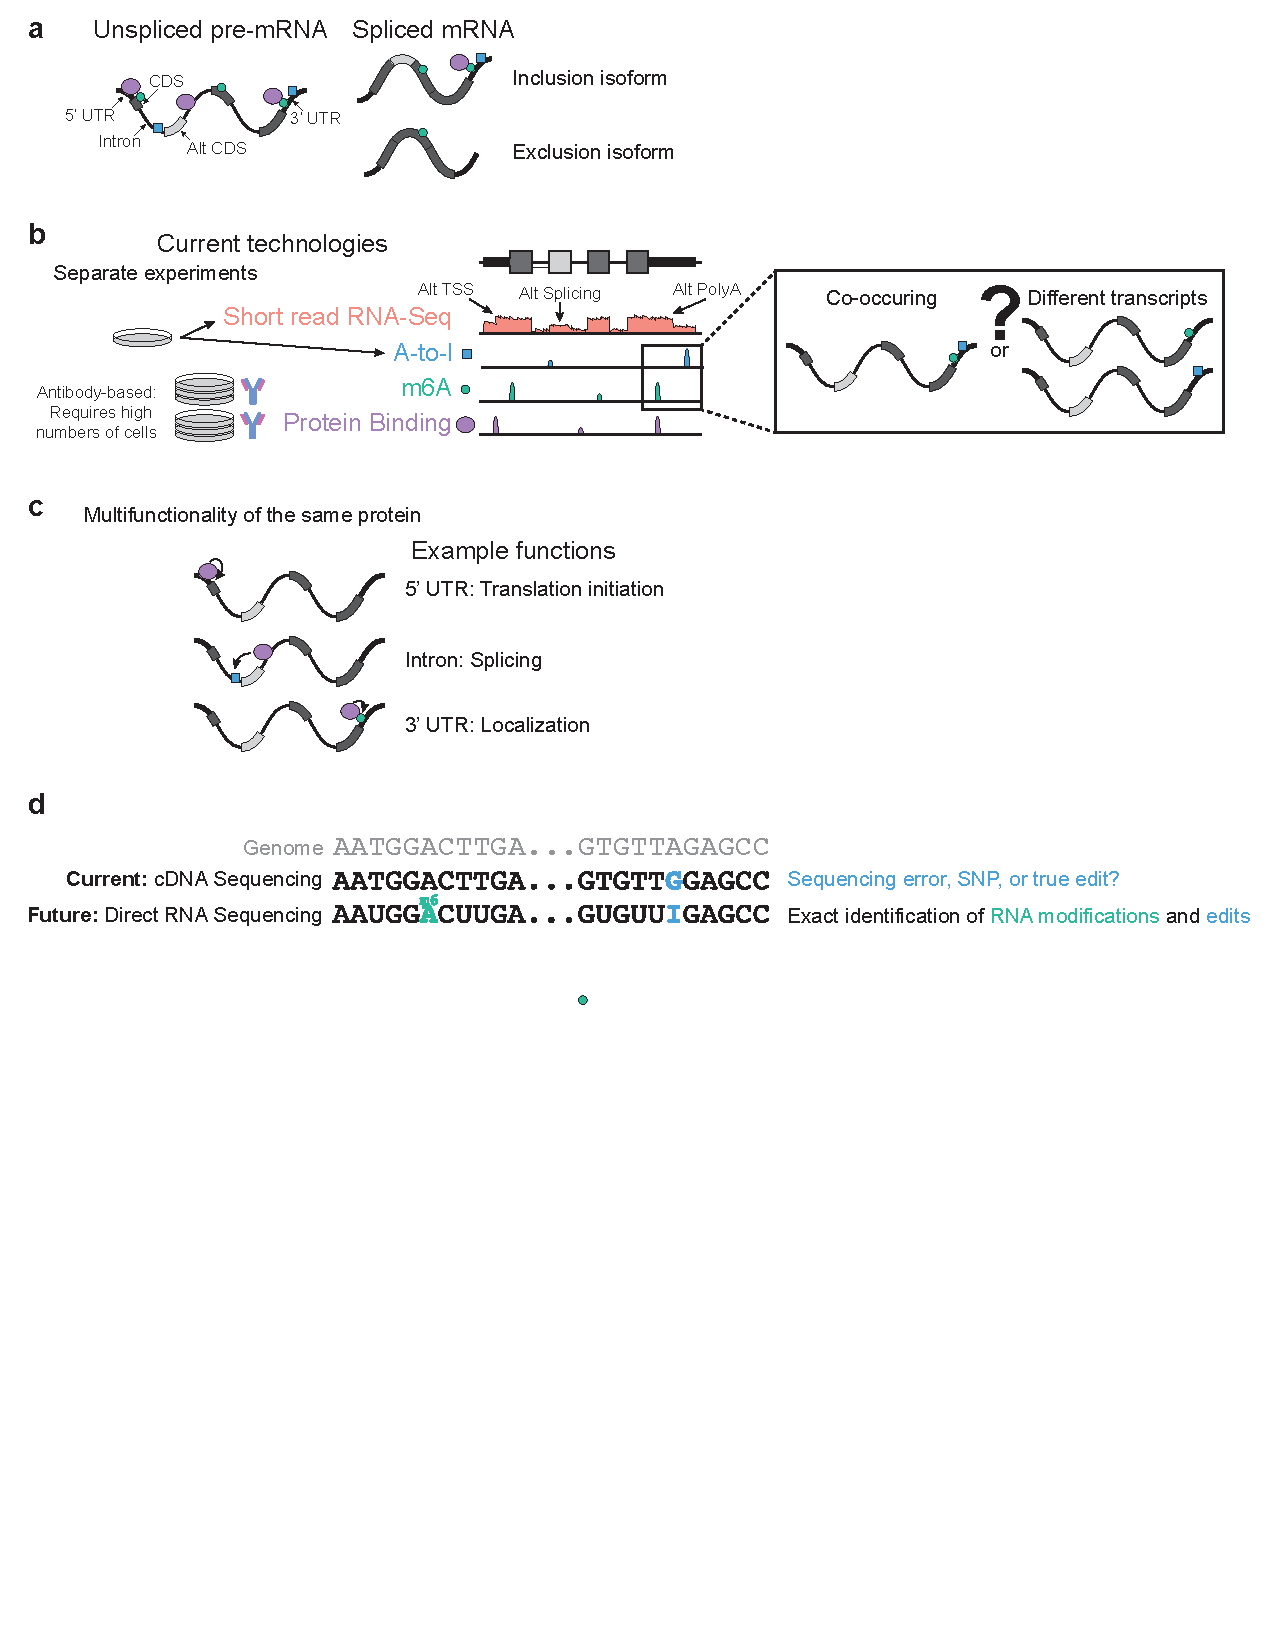
\includegraphics[width=5.8in]{figures/singlecell_future_methods}
  \caption[Unmet needs in RNA processing and potential future technologies.]{Unmet needs in RNA processing and potential future technologies.\\
\textbf{a.}~Left, example RNA transcript with RBPs (purple), A-to-I editing (blue), and m6A (green). Right,  possible inclusion and exclusion isoforms with different post-transcriptional modifications of splicing, m6A, RBP binding, and m6A modification.\\
\textbf{b.}~Current technologies allow for visualization of RNA abundance, A-to-I editing, m6A methylation, and protein binding, but cannot determine whether these occur on physically different or the same molecules.\\
\textbf{c.}~Technologies are needed to investigate multifunctionality of the same protein, e.g. if it performs different functions based on where it binds in the transcripts. Additionally, this would be interesting to study redundancy of different proteins such as splicing factors.\\
\textbf{d.}~Future direct RNA sequencing technologies would allow for direct identification of multiple RNA modifications and edits on the same transcript, unlike currently available technologies.}
\label{fig:singlecell_future_methods}
\end{figure}


Previously, it was thought that there are certain ``uncertainty principles'' in biology, such that one could not know both both the genotype and phenotype of a living cell (Strippoli et al., 2005) or both the cellular ``position'' (current cell state) and ``momentum'' (a cell's past or future, i.e. its lineage or differentiation trajectories) (Shapiro et al., 2013). However, recent work has turned these principles on their head. Both the genotype and phenotype can be measured from a single cell by capturing both DNA and RNA (Macaulay et al., 2015; Reuter et al., 2016), even coupling with measuring DNA methylation and RNA (Angermueller et al., 2016; Hou et al., 2016). A cell's ``position'' and ``momentum'' can be inferred through algorithms that delineate cellular trajectories from phenotypic measurements such as RNA-seq, reviewed thoroughly by (Cannoodt et al., 2016). We expect more technologies to upend traditional thinking of what is possible at the single cell level.

\subsection{Co-occurrence and mutual exclusivity of RNA processing events}

Current technologies to measure transcript abundance and nucleotide modifications, must be performed in separate, bulk experiments, and beyond correlations, the co-occurrence of these [interactions] on the same transcript is unknown (Figure~\ref{fig:singlecell_future_methods}b). Future understanding of the interdependence of RNA processing will require the measurement of multiple aspects of RNA processing at once. This will require is direct RNA sequencing without creation of a cDNA template such as by the Oxford Nanopore MinION (Wanunu et al., 2011) or Pacific Biosciences Single Molecule Real-Time (SMRT) Sequencing (Flusberg et al., 2010). These technologies can directly detect RNA modifications such as m6A and inosine as presence of A-to-I editing (Carr, 2016; Garalde et al., 2016; Saletore et al., 2012). Unfortunately, these technologies are plagued with high error rates and this challenging problem of accuracy for single molecule sequencing will need to be addressed. Nonetheless, as the entire transcript is measured, these would also reveal the co-occurrence on relationships such as between alternative splicing and nucleotide modifications, shedding light on the co-dependence (or independence) of RNA processing elements.
Beyond measuring presence or absence of RNA and its modifications, the interactions of an RNA modification with structure and binding partners will be important. Current methods for measuring RNA secondary structure, typically by selectively measuring only single- or double-stranded RNA, require thousands of cells as input (Bevilacqua et al., 2016; Rouskin et al., 2014; Wan et al., 2011, 2014), thus averaging out the signal across many cells. Scaling these protocols down to single cells will be challenging, it will require tiny amounts of each reaction occurring in nanoliter volumes of captured cells.

\subsection{Spatial analysis: Tissue- and organ-level in vivo}

Disease focus (from Fernando)
ALS
To study ALS, People either extract the entire spinal cord or laser-capture microdissected motor neurons from the spinal cord
Nobody knows what the other cell types do 
How are the supporting glia, astrocytes affected in the ALS spinal cords?
Alzheimer's (from Alex Shishkin)
Market size is Billions of dollars
Hematopoiesis (from Fred)
Niches in the body
Responding to immune insults or lesions
Spatial mapping of the cell of origin with the RNA seq
Spatial mapping of gene expression back to 3d position of cells (Achim et al., 2015; Mori et al., 2017)
Ed boyden's methods
Spatial transcriptomics (Ståhl et al., 2016; Vickovic, 2017) 
Fixed tissue, barcode each location
Then do sequencing and reconstruct
Long Cai's methods (Frieda et al., 2017; Shah et al., 2016a)
Seurat (Satija et al., 2015)
Used known landmark genes
E.g. for a tumor, shave away the outer layer of cells, sequence, and keep going
How are genes differentially expressed?
Outer layer -- more prone to metastasis
Inner layer -- hypoxic

\subsection{Dynamics/time scale}

Most single-cell technologies are destructive -- once you sample the cell, you can't put it back and see how it responds in a new situation
``Single-cell uncertainty principle'' - similar to the ``uncertainty principle'' of measuring genetics in a living cell (Strippoli et al., 2005)
Originally defined for not knowing both the genotype and the phenotype of a living cell
In cellulo labeling of RNA (Custer and Walter, 2016)
Labels RNA fluorescently without adding much molecular weight


\subsection{Moonshot: Spatial + Dynamics}

Moon shot target: live cell imaging
Temporal dynamics could be measured by tracking RNA molecules with RNA-targeted CRISPR/Cas9 (Nelles et al., 2016), provided the technique scaled to the single molecule level.
Biggest problem: signal amplification

Watch assembly of the spliceosome in nuclear speckles in real time
Watch XIST crawl across the X-chromosome in real time
Step 1: live-cell abundance of one RNA
Cas9 + fluorophore
Step 2: Live-cell imaging of multiple RNAs
Cas9 + multiple fluorophores across several RNAs
Step 3: live-cell imaging of different ends of one RNA
Cas9 + multiple fluorophores at beginning, middle and end of the RNA



\subsection{Single cell multi-omics: One cell, many measurements}

A major problem in the field of high-throughput biology is that as soon as a facet of a molecule is digitized, all other context is lost. For example, measuring RNA may inhibit measuring DNA, and measuring RNA abundance cannot currently be performed simultaneously with investigation of nucleotide modifications. How can cellular context be maximized in a high-throughput manner?
This is a problem because the interplay between genotype and phenotype is lost.

One solution to ameliorate the lost context is simultaneous measurements of multiple categories of molecules. While simultaneous capture of the (epi-)genome and transcriptome have been major breakthroughs (Angermueller et al., 2016; Dey et al., 2015; Hou et al., 2016; Macaulay et al., 2015; Reuter et al., 2016), there are many more aspects of cellular state that are still invisible to the sequencing eye. 
Effect of non-RNA on RNA processing - e.g. DNA (chromatin, structure, SNPs) on RNA Processing (quantitative trait loci - QTLs)
Chromatin modifications and their effect on transcription speed and alternative splicing
Quantitative trait loci - SNPs + RNA processing
For example, abundances of proteins or metabolites in conjunction with RNA would provide a fuller picture of cellular state.
E.g. does presence of certain sugars or signaling molecules co-occur with certain RNAs? Discovery of novel signaling pathways
Chromatin structure, along time 4D nucleome (Dekker et al., 2017)
Post-translational modifications of proteins (phosphorylation, glycosylation)
RBPs are glycosylated
Does an RBP bind different regions, perform different functions, or interact with different proteins, when it is differentially glycosylated?
Time scale: phosphorylation can be on the order of seconds

Another method to create additional context for each individual cell is to combine high-throughput measurements with genome editing such as with CRISPR/Cas9, allowing for dissection of complex phenotypes in mammalian cells at large scales. For example, Perturb-seq is a method that combines knockdown of genes using CRISRPi with single-cell RNA-seq, and was used to study the unfolded protein response (Adamson et al., 2016) and effect of lipopolysaccharides on dendritic cells (Dixit et al., 2016). This created a computational scientist's dream dataset, as for each gene that was knocked down, there was a control dataset, and thus for developing algorithms, one could always have a negative control to check with. Perturb-Seq could be applied to study any aspect of RNA processing, e.g. systematically knocking down all protein components of the spliceosome or different alternative splicing factors. 
Another possibility is coupling RNA-seq with lineage-specific barcodes through genome editing by CRISPR/Cas9 (McKenna et al., 2016). This would allow for comparing the transcriptomes of cells from similar lineages. Using phylogenetic techniques, cell lineages could be reconstructed and even the times at which cells asymmetrically divided to change fates could be found. If RNA-seq encodes a cell's present, then its traced lineage encodes its past. This lineage tracing method, coupled with direct RNA sequencing, would help to understand how developmentally regulated RNA processing events such as RNA editing, m6A, and alternative splicing, are finely tuned in different lineages. Do all cells that were committed to a particular lineage also have certain RNA processing events? This could indicate inheritability of the event, either encoded through the genome or by asymmetrically dividing the RNA content of a mother cell.


\section{Discussion}

Previous ‘single-cell' studies were limited to microscopy and other visual tools
Ultimately, ‘single-cell biology' is ‘biology'
Each RNA lives a rich, fulfilled life, and this is difficult to measure through single-cell techniques due to technical limitations.
Many questions remain
How do the many transient aspects of RNA, such as nucleotide modifications, binding partners, 3D structure, and localization, affect each other?
So far has been studied for one transcript, a few modifications
May not even know to study the co-interaction between these aspects on a particular transcript

%   \chapter{The \emph{Expedition} software suite: Computational tools for transcriptome analysis}


% From main text: We developed Expedition, a suite of algorithms integrated in a complete software package designed to address three key concepts that are critical for single-cell analyses: (1) rejection of an alternative event if its definition is incompatible with the data, and (2) ability to describe the variation of AS such as detect bimodality and (3) visualize AS distribution changes from one cell type or state to another.

In this paper, we developed the \emph{Expedition} suite, consisting of  software packages that addressed three key deficiencies in single-cell alternative splicing analysis:

\begin{enumerate}
	\item \textbf{Detect and quantify alternative splicing quickly, with minimum false positives: \outrigger, \Cref{sec:outrigger}}\\
	In single-cell analysis, absolute quantitation of gene expression or ``percent spliced-in'' (Psi/$\Psi$) is important and enable us to learn the distribution of these quantitations. Previously, relative quantitation for splicing ($\Delta\Psi$) is more commonly used to calculate the difference between groups. Such relative quantitation tolerates false positive better, as false positives may not vary between groups, $\Delta\Psi \sim 0$ and are thus not noticeable in pairwise comparisons. However, when studying distribution of absolute quantitation, such false positives obscure the observation in unpredictable way and hinder biological interpretation. The second main problem of previous splicing algorithm is the inflexible definitions of alternative exons. The same alternative exons may utilize different flanking exons in different cells/samples, thus leading to different biological interpretation. To address these problems, we create \outrigger, which uses junction reads to find de novo exons, creates a splice graph to define junction-based alternative events, filters for conserved splice sites, and strictly rejectes cases of alternative events incompatible with the data at hand. Finally, we discuss and compare to the popular MISO\cite{Katz:2010iv} algorithm.
	\item \textbf{Classify modalities of alternative splicing events, including bimodal: \anchor, \Cref{sec:anchor}}\\
	The power of single-cell analyses rises from the ability to study the distribution of a parameter-of-interest. There are a few statistical methods for finding bimodal distributions, but none are sufficient because they are either not sensitive enough, or not robust enough to noise. Additionally, these methods only deal with bimodal distribution and do not classify other distributions, such as unimodal or multimodal. To create a sensitive distribution classifier for all modalities, we used Bayesian methods to create \anchor, and compare our method to a simple binning method, the bimodality index\cite{Wang:2009wm}, and the bimodal dip test\cite{Hartigan:1985ca}.
	\item \textbf{Quantify and visualize dynamics in distributions: \bonvoyage,\linebreak \Cref{sec:bonvoyage}}\\
	While there are many statistical tests to compare changes in distributions, few of them is coupled with visual tools to present changes in distribution with both magnitude and direction. For the specific question of alternative splicing changes, we are interested in observing a event becomes more included or more excluded. Thus we have employed machine learning methods to create a visualizable, interpretable 2d space with ``included'' and ``excluded'' axes. This method is compared to the quantification offered by the Jensen-Shannon Divergence (JSD)\cite{Cover:2011vn}.
\end{enumerate}

\section{\texttt{outrigger}: Splicing estimation with \emph{de novo} annotation and graph traversal}
\label{sec:outrigger}

Currently available tools for AS detection and quanitification have two major problems: (1) inflexible definitions that cannot handle different configurations of flanking exons for the same alternative junctions, and (2) lack of rejection of an alternative event even if its definition is incompatible with the data-at-hand. The first problem is solved with \texttt{outrigger index}, which defines all potential alternative events based on the junctions and alternative exons from the aggregate of entire sample sets in a given project, and enumerates all biologically possible flanking exon combinations. This step maximize the likelihood to identify all possible alternative events. To ensure only valid alternative events were generated, we added \texttt{outrigger validate} to remove alternative events with introns lacking conserved splice sites. The second prolbem is solved with \texttt{outrigger psi}, which applies strict rules to only permit junctions with sufficient coverage for an event in a given sample. All the parameters in the rules can be user-defined. Thus, outrigger addresses key issues with current alternative splicing software.

\subsection{Algorithm overview}

Broadly, the goal of \outrigger\, is to create a custom, \emph{de novo} alternative splicing annotation by using junction reads and exon definitions to create a exon-junction graph, traversing the graph to find alternative events, and calculate percent spliced-in (Psi/$\Psi$) of the alternative exons.


\begin{figure}[h]
  \centering
  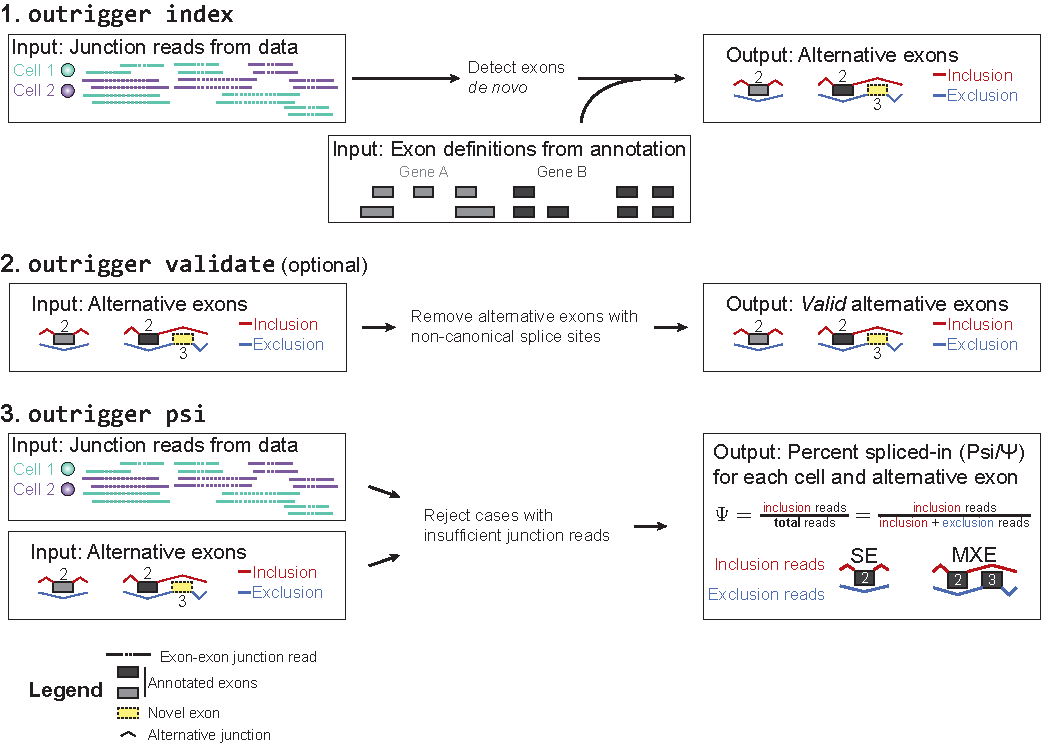
\includegraphics[width=5.6in]{figures/outrigger_overview.pdf}
  \caption[Overview of \outrigger's three steps and associated commands: indexing (\texttt{outrigger index}), validation (\texttt{outrigger validate}) and percent spliced-in (Psi/$\Psi$) calculation (\texttt{outrigger psi})]{Overview of \outrigger's three steps and associated commands: indexing (\texttt{outrigger index}), validation (\texttt{outrigger validate}) and percent spliced-in (Psi/$\Psi$) calculation (\texttt{outrigger psi}). In the first step of building an index, \outrigger\, considers the entirety of junction reads from the user-input dataset to detect exons \emph{de novo}, adds annotated exons, then searches for alternative exons. In the second, optional, step of validating the detected events, \outrigger\, removes alternative exons with flanking introns lacking consensus splice sites. For the third step of calculating Psi/$\Psi$, \outrigger\, utilizes junction reads together with alternative exons defined in the indexing step and calculates $\Psi$ for each sufficiently covered event. Only junction reads are used to represent inclusion or exclusion reads. SE, Skipped Exon; MXE, Mutually Exclusive Exons.
  }
  \label{fig:outrigger_overview}
\end{figure}




% --- BEGIN manual facingcaption --- %
\clearpage
\thispagestyle{facingcaption}
\begin{figure}[h]
\captionsetup{labelformat=prev-page}
  \caption[Internal steps of indexing via \texttt{outrigger index}: Exons identification and defining alternative events.]{
  Internal steps of indexing via \texttt{outrigger index}: Exons identification and defining alternative events.\\
% \captionof{figure}{\textbf{} \\
\textbf{a.} Internal workings of the indexing step via \texttt{outrigger index}. User-provided inputs junction reads can be either genome-aligned \texttt{.bam} files, the \texttt{.SJ.out.tab} splice junction files from the STAR aligner, or a compiled table in \texttt{.csv} of all junction reads from all samples for the project. Step 1, only junction reads with sufficient depth in a cell/sample are retained. By default, the minimum number of reads is $10$ per cell/sample, which can be modified with the flag \texttt{-{}-min-reads}. Step 2, junction reads are used to identify junction locations, and reads are aggregated across all cells/samples regardless of which cell/sample it came from. Step 3, if there is a ``gap'' between two junctions that is smaller than certain length $X$ (by default, $X=100$ nucleotides but can be modified with the flag \texttt{-{}-max-de-novo-exon-length}), then an exon is inserted. Step 4, the identified exons are compared with the annotated exons to obtain the pairwise relationships between exons and junctions. Step 4 outputs a table of ``triples:'' of \texttt{(exon, direction, junction)} encoding the directional relationship between exons and junctions. Step 5, the output tables from step 4 are utilized to connect exons through junctions and creates a graph database. Finally, in Step 6, alternative exons are identified by traversing the graph database. The output of the indexing step run by the command \texttt{outrigger index}, is junction-based, outputting the alternative exon and all possible configurations of flanking exons for each event. For example, on the bottom right, the same skipped exon event using the same alternative junctions, have four possible configurations of flanking exons. They are considered to be the same event, but are reported with all four configurations for the ease-to-use in downstream analysis.\\
\textbf{b.} Defining alternative events and comparison of biological interpretability of events found by MISO and \outrigger. For a given alternative exon (black box), there can be multiple transcripts corresponding to the alternative exon but with different flanking exons. MISO chooses to define the alternative event using the shortest exons on both sides. Yet, this MISO-defined alternative event may not actually exist as a transcript in the dataset and will be misleading to interpret. For example, attempts to translate such non-existing transcript(s) will be inappropriate. In contrast, \outrigger\, defines the event based on the junctions, and outputs all corresponding flanking exon configurations, thus enabling broader use of the outputs and more relevant biological interpretation.
}
\label{fig:outrigger_index}
\end{figure}
\clearpage
\begin{figure}[h]
\ContinuedFloat
\captionsetup{labelformat=empty}
\centering
% \includegraphics[width=5.8in]{sandiego.jpg}
  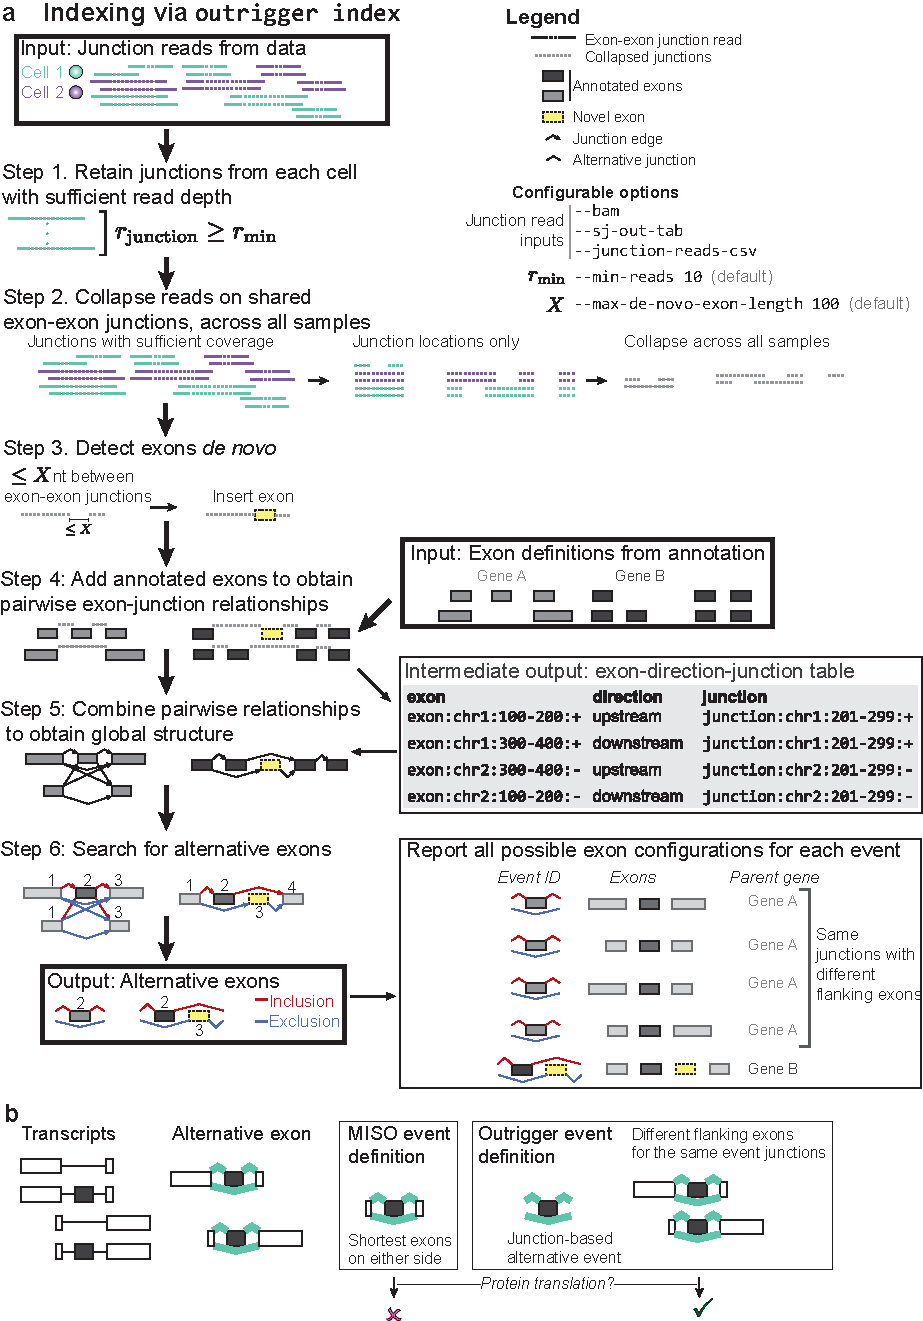
\includegraphics[width=5.8in]{figures/outrigger_index}
\end{figure}
%and, I'm not sure why, but one of the times I used this code the figure number wasn't augmented for the next figure, so check your figure numbers and if necessary uncomment the following line
\addtocounter{figure}{1}
\clearpage
% --- END manual facingcaption --- %


\paragraph{\texttt{outrigger index}: Create custom alternative splicing annotation.} The following is a narrative describing \textbf{\Cref{fig:outrigger_index}a}.


\subparagraph{Inputs.} Two inputs are required for \texttt{outrigger index}: junction counts and gene annotations. The junction counts can be provided in many forms: either \texttt{.bam} \cite{Group:OEYDIUUE} genome alignment files, splice junction count \texttt{.SJ.out.tab} files created by the STAR aligner\cite{Dobin:2013fg}, or a pre-compiled table of samples' junction reads in a \texttt{.csv} format. The gene annotations can be provided in \texttt{.gtf} or \texttt{.gff} format.

\subparagraph{Step 1: Retain junctions from each cell with sufficient read depth.} Junctions with reads in an individual sample less than the minimum number of reads, $r_{\min}$ are removed. By default, $r_{\min} = 10$, and can be adjusted by the user, for example to a minimum of 88 reads, with \texttt{-{}-min-reads~88} on the command line. To illustrate, if one junction is observed with two (2) reads in 100 samples, although there were a total of 200 reads observed on the junction, it will be discarded at this step. Because, there is not sufficient evidence to suggest that this junction is well-covered in any sample.

\subparagraph{Step 2: Collapse reads on shared exon-exon junctions, across all samples.} The aggregate of all junctions from all samples in a given project are create to maximize the likelihood of identifing all potential alternative events.

\subparagraph{Step 3: Detect exons \emph{de novo}.} If the gap between two junctions is under $X$ nucleotides, an exon will be inserted at the gap. This maximum $X$ is necessary, because otherwise we could insert ``exons'' that are many kilobases long, but aren't true exons -{}- they are the intergeneic space between genes. By default, $X = 100$, and this can be adjusted by the user, for example to 157 nucleotides, with the command line flag, \texttt{-{}-max-de-novo-exon-length~157}.

\subparagraph{Step 4: Integrate exon annotation to obtain pairwise exon-junction relationships.} Annotated exons are integrated with the \emph{de novo} exons and create a table of the pairwise relationships of each exon to each junction. We do this by creating a database of genes, transcripts, and exons from a GTF gene annotation file using \texttt{gffutils} \cite{gffutils:sP8uhXuv}, and observing which junctions are adjacent to each exon. This outputs an \emph{``exon-direction-junction''} table which is used in Step 5.

\subparagraph{Step 5: Combine pairwise relationships to obtain global structure.} We then use the adjacencies to build a directional graph which connects exons to each other via junctions. This graph database was built using \texttt{graphlite} \cite{graphlite:vt}, a Python program that provides a lightweight graph wrapper over SQLite.

\subparagraph{Step 6: Search for alternative exons.} To find alternative events, all exons in the graph database were transversed to test, if starting from that exon, it could be a first exon of an skipped exon (SE) or mutually exclusive exon (MXE) event.

\subparagraph{Outputs.} The output of \texttt{outrigger index} is a folder containing the following. The \texttt{events.csv} file contains the event definitions will be used by \texttt{outrigger psi}. The \texttt{exonN.bed} files, where \texttt{N} is an exon number, will be used by \texttt{outrigger validate} to check for canonical or non-canonical splice sites.

The splicing event definitions in the \texttt{events.csv} files are specified by the junctions and the alternative exon. As there may be multiple potential flanking exons with the same junctions, rather than choosing a single version (as is done by MISO, \textbf{\Cref{fig:outrigger_index}b}), we output all possible flanking exon configurations. Thus, while the critical alternative exons are exon 2 for SE events and exons 2 and 3 for MXE events, we show all possible exon flanking exon 1s and exon 3s for SE, and all possible flanking exon 1s and exon 4s for MXE events (\textbf{\Cref{fig:outrigger_index}a}, lower right).

Below is an example command using \texttt{outrigger index}:

\begin{verbatim}
outrigger index --bam *sorted.bam \
    --gtf gencode.vM10.annotation.gtf
\end{verbatim}

This creates a folder called \texttt{outrigger\_output} with the following contents:


\begin{figure}
\footnotesize
\dirtree{%
.1 outrigger\_output/.
.2 index.
.3 gtf\DTcomment{Added by Step 3}.
.4 gencode.vM10.annotation.gtf\DTcomment{Added by Step 4}.
.4 gencode.vM10.annotation.gtf.db\DTcomment{Added by Step 4}.
.4 novel\_exons.gtf\DTcomment{Added by Step 3}.
.3 exon\_direction\_junction.csv\DTcomment{Added by Step 4}.
.3 mxe\DTcomment{Added by Step 6}.
.4 event.bed\DTcomment{Added by Step 6}.
.4 events.csv\DTcomment{Added by Step 6}.
.4 exon1.bed\DTcomment{Added by Step 6}.
.4 exon2.bed\DTcomment{Added by Step 6}.
.4 exon3.bed\DTcomment{Added by Step 6}.
.4 exon4.bed\DTcomment{Added by Step 6}.
.4 intron.bed\DTcomment{Added by Step 6}.
.3 se\DTcomment{Added by Step 6}.
.4 event.bed\DTcomment{Added by Step 6}.
.4 events.csv\DTcomment{Added by Step 6}.
.4 exon1.bed\DTcomment{Added by Step 6}.
.4 exon2.bed\DTcomment{Added by Step 6}.
.4 exon3.bed\DTcomment{Added by Step 6}.
.4 intron.bed\DTcomment{Added by Step 6}.
.2 junctions\DTcomment{Added by Step 1}.
.3 metadata.csv\DTcomment{Added by Step 2}.
.3 reads.csv\DTcomment{Added by Step 1}.
}
\caption{Example output of \texttt{outrigger index} command.}
\end{figure}


Besides outputting the relevant \texttt{events.csv} which is used in \texttt{outrigger psi} to define events, we also output \texttt{.bed} files for the entire event, the alternative intron, and each exon, facilitating downstream sequence analysis.


\paragraph{\texttt{outrigger validate}: Remove alterantive splicing lacking conserved splice sites.} The following describes the biological intuition behind \textbf{\Cref{fig:outrigger_validate_frankenevents}a}. Major (U2) splicesome recognize splice-sites as  ($5^\prime$ end of intron/$3^\prime$ end of intron) \texttt{GT/AG} and \texttt{GC/AG} the Minor (U12) spliceosome recognizes splice-sites as \texttt{AT/AC}\cite{McManus:2011en,GarciaBlanco:2004kl}. By default, these combinations of splice-sties are allowed. But the valid splice sites can be user-specified and changed for example to \texttt{AA/AA} and \texttt{GG/GG} with \texttt{-{}-valid-splice-sites~AA/AA,GG/GG}.

The output of \texttt{outrigger validate} is a \texttt{splice\_sites.csv} folder containing the splice sites, and an additional folder in the splice type folder, called \texttt{validated}, containing filtered \texttt{events.csv} which only contain alternative events with valid splice sites. For example, as a follow up on our previous \texttt{outrigger index} command, we validate the alternative exons with the command,

\begin{verbatim}
outrigger validate -{}-genome mm10 \
    -{}-fasta GRCm38.primary_assembly.genome.fa
\end{verbatim}

This creates the following additions to the \texttt{outrigger\_output} folder:

\begin{figure}
\footnotesize
\dirtree{%
.1 outrigger\_output/.
.2 index.
.3 gtf.
.4 gencode.vM10.annotation.gtf.
.4 gencode.vM10.annotation.gtf.db.
.4 novel\_exons.gtf.
.3 exon\_direction\_junction.csv.
.3 mxe.
.4 event.bed.
.4 events.csv.
.4 exon1.bed.
.4 exon2.bed.
.4 exon3.bed.
.4 exon4.bed.
.4 intron.bed.
.4 splice\_sites.csv\DTcomment{Added by \texttt{outrigger validate}}.
.4 validated\DTcomment{Added by \texttt{outrigger validate}}.
.5 events.csv\DTcomment{Added by \texttt{outrigger validate}}.
.3 se.
.4 event.bed.
.4 events.csv.
.4 exon1.bed.
.4 exon2.bed.
.4 exon3.bed.
.4 intron.bed.
.4 splice\_sites.csv\DTcomment{Added by \texttt{outrigger validate}}.
.4 validated\DTcomment{Added by \texttt{outrigger validate}}.
.5 events.csv\DTcomment{Added by \texttt{outrigger validate}}.
.2 junctions.
.3 metadata.csv.
.3 reads.csv.
}
\caption{Example output of \texttt{outrigger validate} command.}
\end{figure}


\paragraph{Potential ``Franken-events'' created by combining junctions over multiple datasets.} As many junctions may occur spuriously in a single cell (sample), aggregating all junctions across all cells (sample) may create events that were not observed in any individual cell (\Cref{fig:outrigger_validate_frankenevents}b). We wanted to ensure we strictly defined when events were valid or not in these cases.

In the case of SE events, the exon will have $\Psi = \text{NA}$ for the cell with the observed inclusion junctions, since they don't have sufficient reads on both sides of the exon. For the cell with the exclusion junction, it will have $\Psi = 0$ since no inclusion reads were observed.

For MXE events, if each of the four junctions was observed independently in a different cell, then all of the cells will have $\Psi = \text{NA}$ for that splicing event since there are no cells which have sufficient reads on all junctions of either isoform.

\begin{figure}
  \centering
  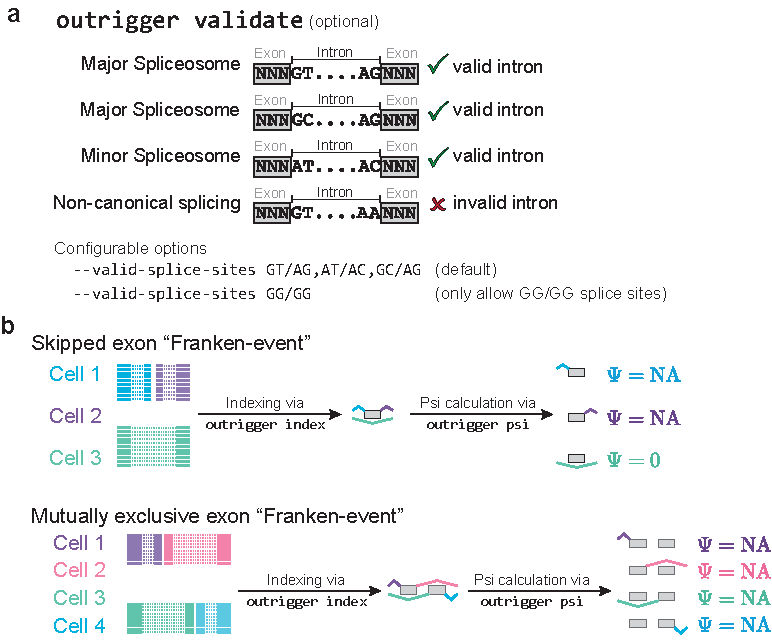
\includegraphics[width=5.8in]{figures/outrigger_validate}
  \caption[\outrigger\, validation and pathological cases.]{
  \outrigger\, validation and pathological cases.\\
\textbf{a.}~Validation via \texttt{outrigger validate}: Removal of alternative events with introns lacking consensus splice sites. In this optional step, exons with flanking introns lacking known splice site motifs are removed. This is configurable. By default, the valid splice sites are specified as, \texttt{-{}-valid-splice-sites GT/AG,GC/AG,AT/AC}, but can be any pair of two nucleotides.\\
\textbf{b.}~Possible pathological cases of \texttt{outrigger}. These ``Franken-events'' consist of junctions that were observed in independent samples. At the indexing step, aggregated reads from multiple cells/samples are considered to construct an index of all junctions to maximize the number of AS events. Yet, at the Psi/$\Psi$ calculation step, in each individual cell/sample, insufficient reads may be observed for certain junction resulting in $\Psi=\text{NA}$ in some cells/samples for the same event. Top, skipped exons, if each junction is observed only in one cell, the cell with the exclusion junction is assigned a $\Psi=0$ while the remaining cells are assigned as $\Psi=\text{NA}$. Bottom, mutually exclusive exons, $\Psi=\text{NA}$ for all 4 cells, as there is insufficient evidence of exon inclusion or exclusion in any one cell. Thus, the number of detected events output by \texttt{outrigger index} can greatly overestimate the number of valid events in the dataset found by \texttt{outrigger psi}.
}
\label{fig:outrigger_validate_frankenevents}
\end{figure}



\paragraph{\texttt{outrigger psi}: Calculate percent spliced-in of alternative exons}

To calculate percent spliced-in (Psi/$\Psi$) of a potentially alternative exon identified in \texttt{outrigger index}, we use the equation for $\Psi= \frac{\text{inclusion reads}}{\text{total reads}}$ \cite{Wang2008-xh}, with substantial checks for whether the event is valid (\textbf{\Cref{fig:outrigger_psi}}). For SE, there is only one exclusion junction and thus the the exclusion junction is weighted by two to compensate (Eq.~\Cref{eq:se_psi}). For MXE, the calcluation is simply the inclusion reads divided by the total reads (Eq.~\Cref{eq:mxe_psi}). The junction reads between exon $i$ and exon $j$ are presented as $r_{i,j}$, displaying inclusion reads in red and exclusion reads in blue.

\begin{multicols}{2}
\noindent
  \begin{gather}
  \text{SE $\Psi$}\nonumber\\
\Psi = \frac{\textcolor{inclusion}{r_{1,2}} + \textcolor{inclusion}{r_{2,3}}}{\textcolor{inclusion}{r_{1,2}} + \textcolor{inclusion}{r_{2,3}} + 2\textcolor{exclusion}{r_{1,3}}} \label{eq:se_psi} %\nonumber
\end{gather}
% \break
\begin{gather}
  \text{MXE $\Psi$}\nonumber\\
\Psi = \frac{\textcolor{inclusion}{r_{1,2}} + \textcolor{inclusion}{r_{2,4}}}{\textcolor{inclusion}{r_{1,2}} + \textcolor{inclusion}{r_{2,4}} + \textcolor{exclusion}{r_{1,3}} + \textcolor{exclusion}{r_{3,4}}} \label{eq:mxe_psi} %\nonumber
\end{gather}
\end{multicols}

Multiple validation steps were incorporated to ensure that the junction reads observed in each sample are consistent with the type of splicing event annotated by \outrigger. This process is described in \textbf{Supplementary Software .~\Cref{fig:outrigger_psi}}.

% --- BEGIN manual facingcaption --- %
\clearpage
\thispagestyle{facingcaption}
\begin{figure}[h]
\captionsetup{labelformat=prev-page}
  \caption[Cases created by percent spliced-in calculation via the command \texttt{outrigger psi}.]{
  Cases created by percent spliced-in calculation via the command \texttt{outrigger psi}.\\
% \captionof{figure}{\textbf{}
The table describes the 11-step sequential logic of \outrigger\, to reject an event in a cell/sample based on that cell/sample's junction reads. If an event reaches a $\Psi=\text{NA}$ case, then it is rejected from that sample, otherwise, it continues through the cases. If the event is rejected, then it is assigned $\Psi = \text{NA}$, if it is not rejected, then it gets a $0\leq \Psi \leq 1$ value based on the junction reads.\\
Strict evaluation of percent spliced-in (Psi/$\Psi$). To compute the percent spliced-in (Psi/$\Psi$) of skipped exon (SE) and mutually exclusive exons (MXE) alternative events during the execution of the command \texttt{outrigger psi}, we use $\Psi= \frac{\text{inclusion reads}}{\text{total reads}}$. We represent the number of reads spanning the junction between exon$_i$ and exon$_j$ as $r_{i,j}$.
}
\label{fig:outrigger_psi}

\end{figure}
\clearpage
\begin{figure}[h]
\ContinuedFloat
\captionsetup{labelformat=empty}
\centering
% \includegraphics[width=5.8in]{sandiego.jpg}
  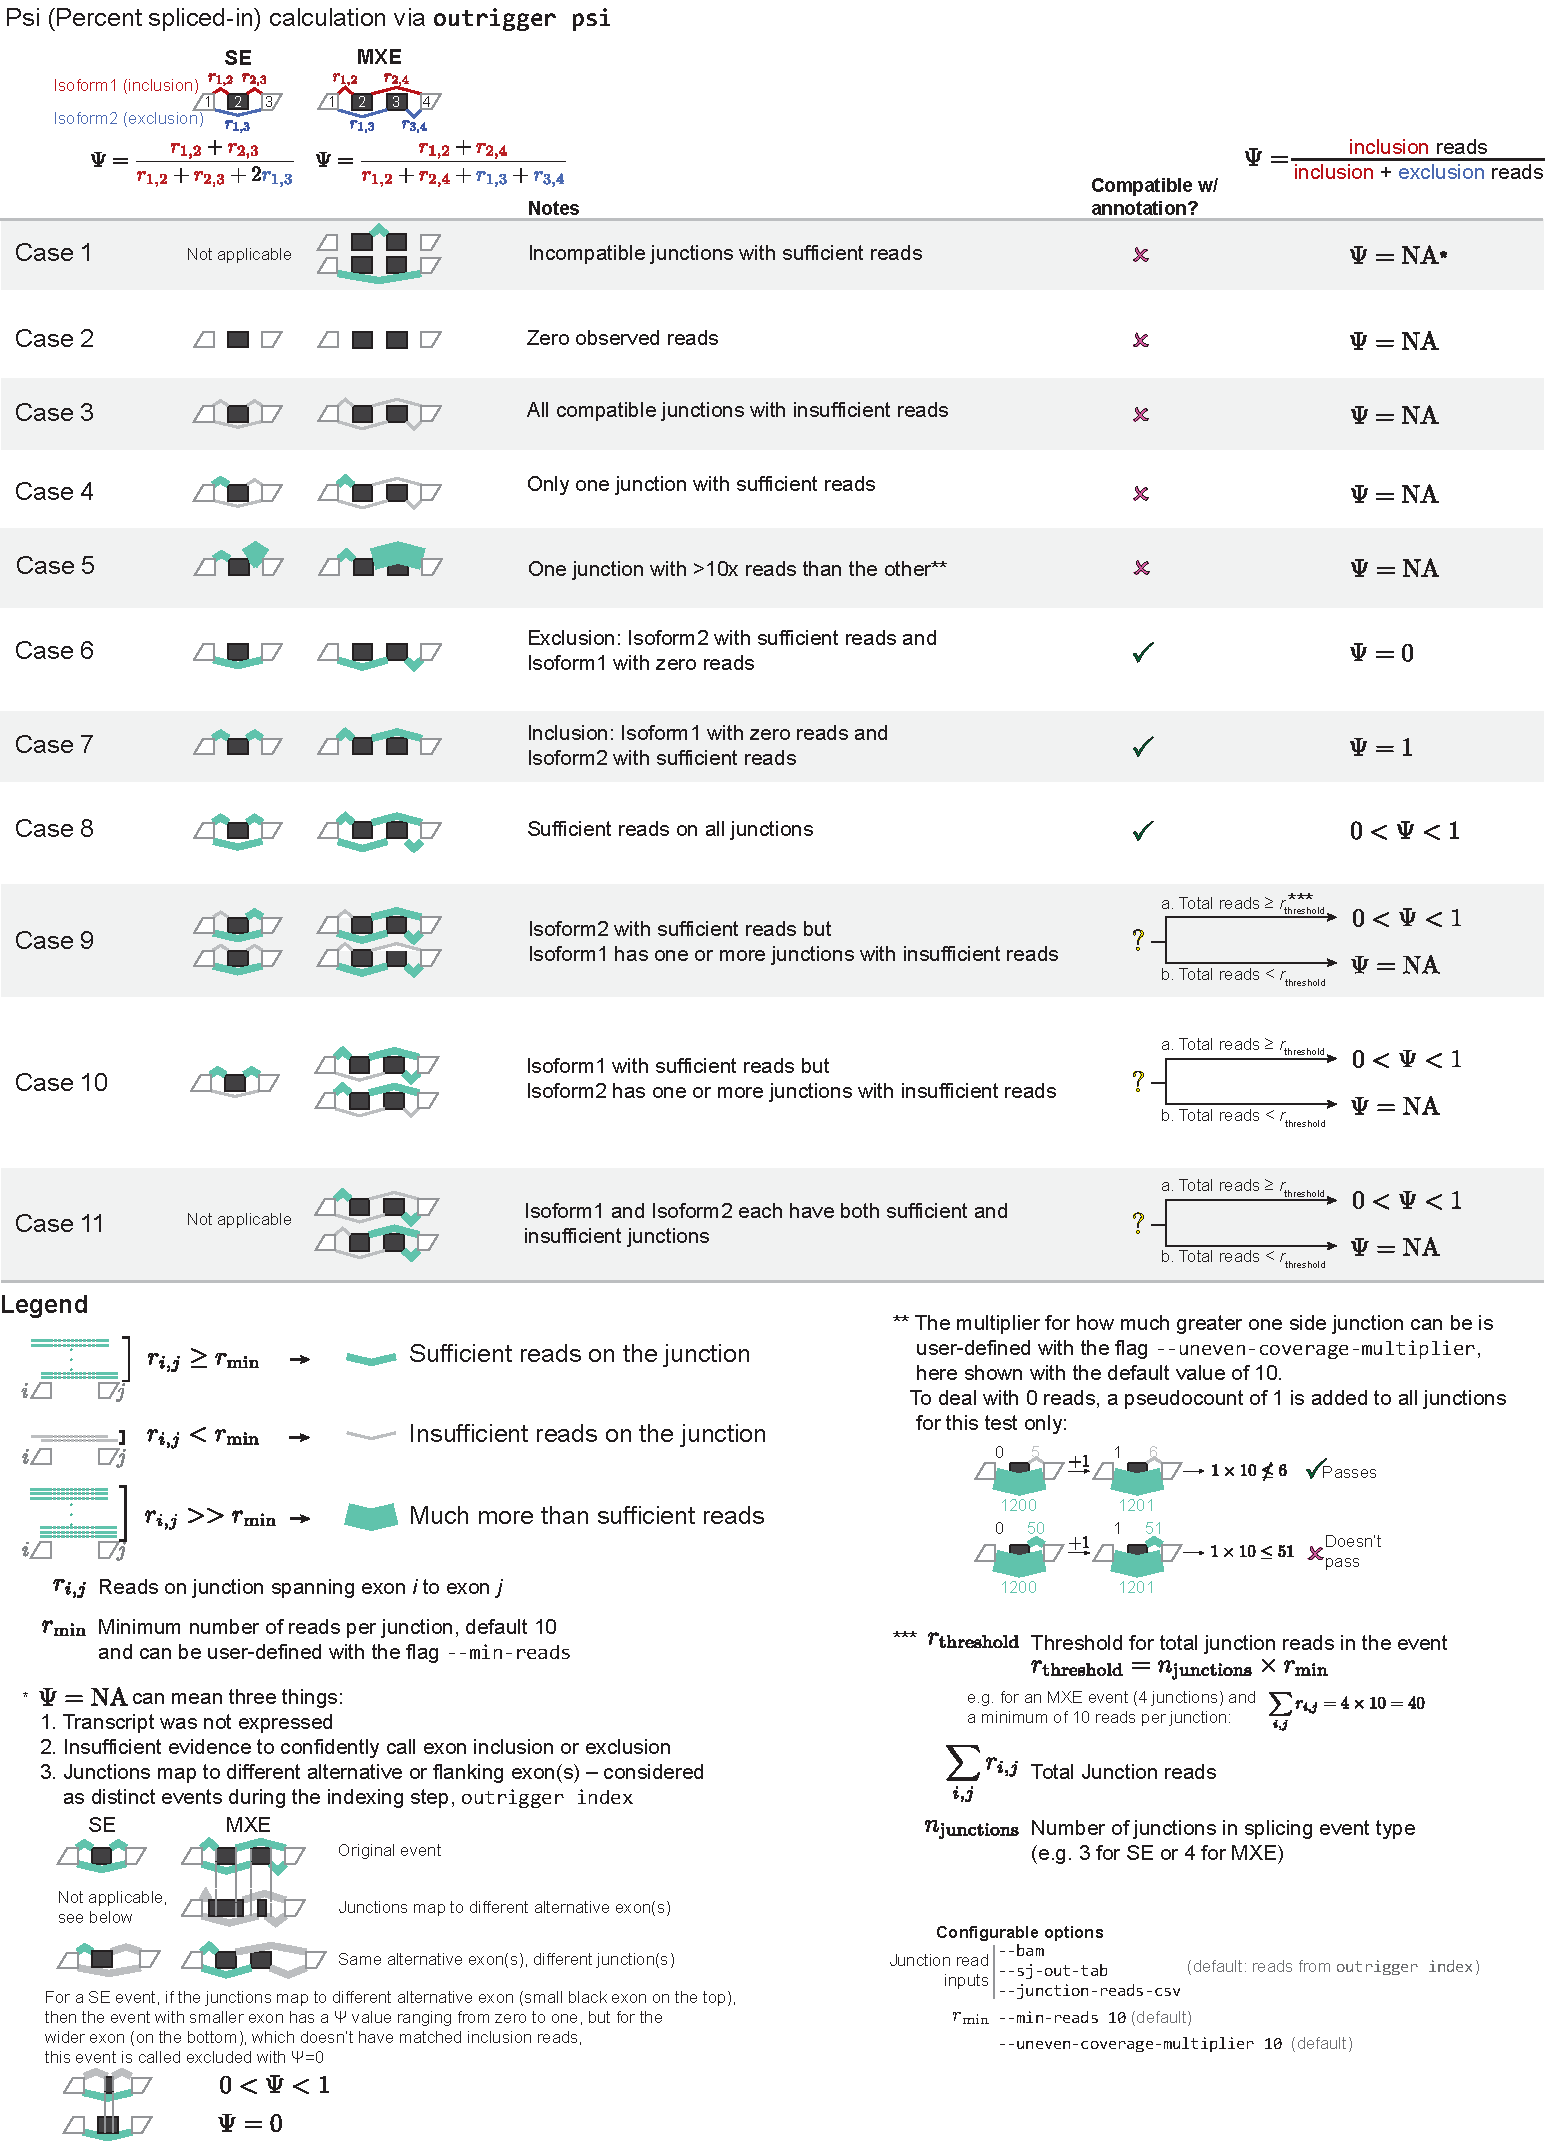
\includegraphics[width=5.8in]{figures/outrigger_psi}
\end{figure}
%and, I'm not sure why, but one of the times I used this code the figure number wasn't augmented for the next figure, so check your figure numbers and if necessary uncomment the following line
\addtocounter{figure}{1}
\clearpage
% --- END manual facingcaption --- %

\begin{longdescription}
	\item[Case 1: Incompatible junctions with sufficient reads.] This step checks whether the junction reads are compatible with a MXE event, or rather a twin cassette event. Specifically, evidence of  $r_{2,3} > r_{\min}$ or $r_{1,4} > r_{\min}$ suggests this junction is a twin cassette event but not an MXE event. In such cases, $\Psi = \text{NA}$. As described in \texttt{outrigger index}, the minimum number of reads is user-defined, for example to 37 with \texttt{-{}-min-reads~37}.
	\item[Case 2: Zero observed reads.] Given no reads is observed, this event is $\Psi = \text{NA}$, rather than $\Psi=0$ since $\Psi=0$ indicates exclusion.
	\item[Case 3: All compatible junctions with insufficient reads.] No single junction has the minimum number of reads $r_{\min}$, by default $r_{\min}$ is 10, and can be modifiable by the \texttt{-{}-min-reads} flag. If this is the case, we assign $\Psi = \text{NA}$.
	\item[Case 4: Only one junction with sufficient reads.] This applies to a single junction of two junctions per isoform, e.g. Isoform2 of either SE or MXE events, and Isoform1 of an MXE event, has sufficient reads. Since only one junction has the minimum number of reads, $r_{\min}$, no sufficient evidence indicates inclusion of exon-of-interest, thus, we assign $\Psi = \text{NA}$.
	\item[Case 5: One junction with $>10\times$ more reads than the other.] When the alternative exon is covered on the two sides with junction reads of great disparity, there is insufficient evidence supporting the inclusion of alternative exon or suggests the exon may involved in a complex splicing, rather than a SE or MXE. Thus, $\Psi = \text{NA}$. The default multiplier is 10 and can be modified by the user, for example to 55 by \texttt{-{}-uneven-coverage-multiplier~55}.
	\item[Case 6: Exclusion: Isoform2 with sufficient reads and Isoform1 with zero reads.] All junctions on Isoform2 have greater than the minimum reads $r_{\min}$, and all junctions of Isoform1 have no observed reads, thus $\Psi = 0$.
	\item[Case 7: Inclusion: Isoform2 with zero reads and Isoform1 with sufficient reads.] All junctions on Isoform2 have no observed reads and all junctions of Isoform1 have greater than the minimum reads $r_{\min}$, thus $\Psi = 1$.
	\item[Case 8: Sufficient reads on all junctions.] Both Isoform1 and Isoform2 have greater than the minimum reads on all their junctions. This is the best possible case for alternative splicing.
	\item[Case 9: Isoform2 with sufficient reads but Isoform1 has one or more junctions with insufficient reads.] If the exclusion isoform, Isoform2 has sufficient reads, but the inclusion isoform (Isoform1) does not, then we assess whether the total read coverage of the event, $\sum_{i,j} r_{i,j}$exceeds $r_{\text{threshold}}$. If so, a $\Psi$ is calculated; if not, $\Psi = \text{NA}$. We define $r_{\text{threshold}}$ as the number of junctions $n$ times the minimum number of reads $r_{\min}$. For example, with a minimum read count is 10 on an SE event, $r_{\text{threshold}} = 30$. For a minimum read count of 10 on an MXE event, $r_{\text{threshold}} = 40$.
	\item[Case 10: Isoform2 has one or more junctions with insufficient reads but Isoform1 has sufficient reads.] Similar to Case 9, we again test if the total read coverage is sufficient to calculate $\Psi$, i.e. if $\sum_{i,j} r_{i,j} \geq r_{\text{threshold}}$. If so, we calculate $\Psi$, and if not, we assign $\Psi = \text{NA}$.
	\item[Case 11: Isoform1 and Isoform2 each have both sufficient and insufficient junctions.] This case only applies to MXE events as SE events have as single Isoform2 junction, and cannot have both sufficient and insufficient junctions. If by the per-junction coverage, it is unclear whether the event has sufficient coverage, then we test if the total coverage of the event is sufficient. If so, we calculate $\Psi$, and if not, we assign $\Psi = \text{NA}$.
\end{longdescription}


% Before we calculate $\Psi$, we ensure that a sample has a valid SE event by checking for enough reads on either both the inclusion junctions ($r_{1,2}$ and $r_{2,3}$) or the exclusion junction ($r_{1,3}$). This protects against calculating $\Psi$ for events that aren't truly SE or MXE events, for example, an alternative first exon event that was annotated as an SE event would have $r_{1,2} = 0$, and thus we wouldn't calculate $\Psi$. For MXE events, we check that there are no reads between exons 2 and 3 ($r_{2,3}=0$), because if there are any reads here, then this is evidence that in a particular sample, this is a twin casette event rather than an MXE event (\textbf{Supplementary \Cref{fig:outrigger_psi}}). For SE events, we also check that for inclusion, there must be $>10$ reads on both sides of the alternative exon, and if there aren't, then we discard the event.
\subparagraph{Outputs} The output of \texttt{outrigger psi} is added into the \\\texttt{outrigger\_output} folder by creating a \texttt{psi} folder for each splice type. \texttt{psi.csv} contains $\Psi$ in a matrix, and the \texttt{summary.csv} produces a summary of all the events observed in all samples with their junction reads.

To follow up with our \texttt{outrigger index} and \texttt{outrigger validate} commands, we can run the below example command in the same directory:

\begin{verbatim}
outrigger psi
\end{verbatim}

This command adds to the existing output folder \texttt{outrigger\_output}. Therefore, we don't need to specify a genome location or reads or index location if this command is run from the same folder as the \texttt{outrigger index} command was run, and there exists in the directory a folder called \texttt{outrigger\_output}.

\begin{figure}
\footnotesize
\dirtree{%
.1 outrigger\_output/.
.2 index.
.3 gtf.
.4 gencode.vM10.annotation.gtf.
.4 gencode.vM10.annotation.gtf.db.
.4 novel\_exons.gtf.
.3 exon\_direction\_junction.csv.
.3 mxe.
.4 event.bed.
.4 events.csv.
.4 exon1.bed.
.4 exon2.bed.
.4 exon3.bed.
.4 exon4.bed.
.4 intron.bed.
.4 splice\_sites.csv.
.4 validated.
.5 events.csv.
.3 se.
.4 event.bed.
.4 events.csv.
.4 exon1.bed.
.4 exon2.bed.
.4 exon3.bed.
.4 intron.bed.
.4 splice\_sites.csv.
.4 validated.
.5 events.csv.
.2 junctions.
.3 metadata.csv.
.3 reads.csv.
.2 psi.\DTcomment{Added by \texttt{outrigger psi}}.
.3 mxe\DTcomment{Added by \texttt{outrigger psi}}.
.4 psi.csv\DTcomment{Added by \texttt{outrigger psi}}.
.4 summary.csv\DTcomment{Added by \texttt{outrigger psi}}.
.3 outrigger\_psi.csv\DTcomment{Added by \texttt{outrigger psi}}.
.3 se\DTcomment{Added by \texttt{outrigger psi}}.
.4 psi.csv\DTcomment{Added by \texttt{outrigger psi}}.
.4 summary.csv\DTcomment{Added by \texttt{outrigger psi}}.
}
\caption{Example output of \texttt{outrigger psi} command.}
\end{figure}

\paragraph{Advantages and limitations of \outrigger.}

The main advantages of \outrigger\, are speed and conserved memory footprint. As \outrigger\, operates only on junction reads, rather than resampling reads from a \texttt{.bam} alignment file, which can range in size from 500MB to 20GB and results in a high memory footprint, \texttt{outrigger} summarizes each \texttt{.bam} file to only its junction reads and uses that to estimate Psi/$\Psi$ values. Additionally, employing three steps of \outrigger\, \outrigger\ is able to maximize the number of potential alternative events and subsequently apply strict validation rules in the step of outrigger psi calculation to eliminate false positive events from each sample.
However, currently, \outrigger\ can only deal with SE and MXE events. We are in the process of incorporating other alternative splice types.

% \subsection{PCR duplicate removal studies}

% We also compared outrigger's performance on pre- and post-duplicate removed dataset. After duplicate-removal, ~93\% events were retained by requiring that each junction is covered by at least 10 unique reads (\textbf{Supplementary \Cref{fig:splicing_qc}f}). When comparing the Psi scores before and after duplicate-removal, the vast majority of events have a consistent Psi within |delta Psi| < 0.2 and only ~7\% are designated as NA in the latter (\textbf{Supplementary \Cref{fig:splicing_qc}h-i}), likely due to the reduced read coverage.

\subsection{Comparison to other methods}

In comparison to the popular splicing program MISO\cite{Katz:2010iv}, \outrigger\, has three major advantages:

\begin{enumerate}
	\item Ability to build de novo exon indexes (\texttt{outrigger index})
	\item Flexiblity of junction-based definitions of alternative exons, enumerating all possible flanking exons (\texttt{outrigger index})
	\item Ability to eliminate incompatible alternative events (\texttt{outrigger psi})
	\item Speed of evaluation. Instead of using the huge \texttt{.bam} alignment files directly, \outrigger\, summarizes the files as junction reads, leading to much faster calculation of percent spliced-in. Once an index is built with \texttt{outrigger index} (24-48 hours), then calculation of $\Psi$/Psi takes 2-4 hours, even on hundreds of samples. With MISO, the calculation can take 8 hours per sample.
\end{enumerate}


\paragraph{Ability to build de novo exon indexes.} MISO provides pre-built alternative splicing indexes, which may not be incompatible with the data at hand. There is a program, GESS \cite{Ye:2014cd} to detect alternative exons from \texttt{.bam} files, which can only handle a handful files at a time and freeze when given hundreds of single-cell \texttt{.bam} files. In contrast, in the outrigger indexing step, \outrigger\,builds indexes based on provided data, which will be integrated with provided exon annotation allowing identification of novel exons.

\paragraph{Flexiblity of junction-based definitions of alternative exons, enumerating all possible flanking exons.} Multiple possible flanking exons can be associated with an alternative exon, most algorithms, including MISO and rMATS \cite{Shen2014-zq}, choose a single set (often the shortest one), rather than being flexible and allowing the user to choose the relevant ones. The resulting ``best guess'' of the alternative event may not be biologically relavent and may be misleading to interprete. In such case, computational translation of alternative events, as demonstrated in Figure 4, will not be possible.

\paragraph{Ability to eliminate incompatible alternative events} Comparing MISO $\Psi$ values side-by-side with a corresponding \texttt{outrigger psi} calculation, we find that $46\%$ of MISO $\Psi$ values are rejected and assigned $\Psi = \text{NA}$ by \outrigger\, (\textbf{\Cref{fig:miso}}).

A large group of false positives that are correctly rejected by \outrigger\, are Case 1, where only incompatible junctions present sufficient reads. For example, when twin cassette events are annotated as MXE events and the data indicates inclusion of both alternative exons, MISO will calculate $\Psi$ as 0.5. Because MISO uses a prior of $\Psi=0.5$ and resamples the data to calculate $\Psi$. In such a case, MISO is never convinced that $\Psi$ should be towards 1 or 0 and remains at $\Psi~0.5$ (\textbf{\Cref{fig:miso}a}). %As a result, these false positive MXE events make up a far larger proportion of the middle modality when using MISO data than with \outrigger\, (\textbf{\Cref{fig:miso}e-f}).

% --- BEGIN manual facingcaption for MISO figure --- %
\clearpage
\thispagestyle{facingcaption}
\begin{figure}[h]
\captionsetup{labelformat=prev-page}
  \caption[Examples of inconsistencies in MISO's estimation with single-cell data.]{Examples of inconsistencies in MISO's estimation with single-cell data.\\
\textbf{a-c}. Representative examples of SE and MXE AS events measured by MISO, but were unsupported with visual inspection on IGV browser, and were disqualified by \outrigger. To identify SE and MXE events, \outrigger\, constructs a \emph{de novo} splicing index based on the junction reads in all libraries in the dataset (see details in \textbf{Figures~\cref{fig:outrigger_index,fig:outrigger_psi,fig:outrigger_validate_frankenevents}}). The following examples are not considered by \outrigger as true SE or MXE events, therefore annotated as NA. Note, MISO does not estimate modality for each event, \anchor\, (see details in \textbf{\Cref{fig:anchor_overview,fig:anchor_simulations_perfect_modalities,fig:anchor_simulations_maybe_bimodals}}) was used to estimate modality.\\
\textbf{a.} Top, a MISO-annotated MXE event in ARF4 with MISO estimated $\Psi$s $\sim0.5$ and classified as ``middle'' modality in each of iPSC, NPC, and MN by \anchor. Yet, in the IGV browser (bottom), this event appears as a twin cassette event, where both exons 2 and 3 are included, indicating that at least in our dataset this event is not consistent with the MISO annotation. Outrigger disqualifies this event as a MXE and assign NA (top left).\\
\textbf{b.} Top, a MISO-annotated SE event in CLF1 with MISO estimated $\Psi$s ranging from $0.1$ to $0.6$ and is classified as a ``middle'' modality event by \anchor\, in each of iPSC, NPC, and MN.  Yet, in the IGV browser (bottom), exon 1 for this annotation is not covered at all. Given the data, outrigger\ do not consider this as a bona fide SE event and assign NA to this event.\\
\textbf{c.} Top, a MISO-annotated MXE event in AHSA1 with a wide range of MISO calculated $\Psi$s and is classified as the ``multimodal'' modality in each of iPSCs, NPC, and MN populations by \anchor. Bottom, in the IGV browser. Exons 2 and 3 are the annotated alternative exons for MXE, however, another two well-covered exons between exon 2 and 3 were observed and one extra exon between exon 3 and 4, which disqualify this event as an MXE event. Furthermore, when both exon 2 and 3 are included, MISO estimated $\Psi$ scores are closer to 1 instead of around $0.5$, as was seen in (\textbf{a}). Thus, outrigger rejects this as MXE and assign NA.\\
\textbf{d.}~Using \outrigger\,'s strict rules on MISO annotations, the majority (51\%) of the data generated by MISO was rejected by \outrigger\, (left). Right, using the exact same annotation from MISO, \outrigger\, 22\% of events found by \outrigger\, had too wide of a confidence interval ($>0.4$) by MISO.\\
\textbf{e.}~Heatmap comparing the numbers and percentages of alternative events that were within $|\Delta\Psi| < 0.2$, switched to exactly 1 or 0 in \outrigger, were NA in either MISO or \outrigger, or were in another case.\\
\textbf{f.}~Barplot of the number of cases found only in MISO (orange) and rejected as NA by \outrigger, and of the cases found only by \outrigger (green) and considered to have too wide of a confidence interval by MISO.\\
To summarize, \texttt{outrigger} follows strict rules to identify alternative splicing (\textbf{Figures~\cref{fig:outrigger_index,fig:outrigger_psi,fig:outrigger_validate_frankenevents}}) and provides a $\Psi$ distribution more localized at the extremes of $\Psi = 0$ and $\Psi = 1$. Although \texttt{outrigger}, may identify fewer events, they are true SE and MXE events.}
\label{fig:miso}
\end{figure}
\clearpage
\begin{figure}[h]
\ContinuedFloat
\captionsetup{labelformat=empty}
\centering
% \includegraphics[width=5.8in]{sandiego.jpg}
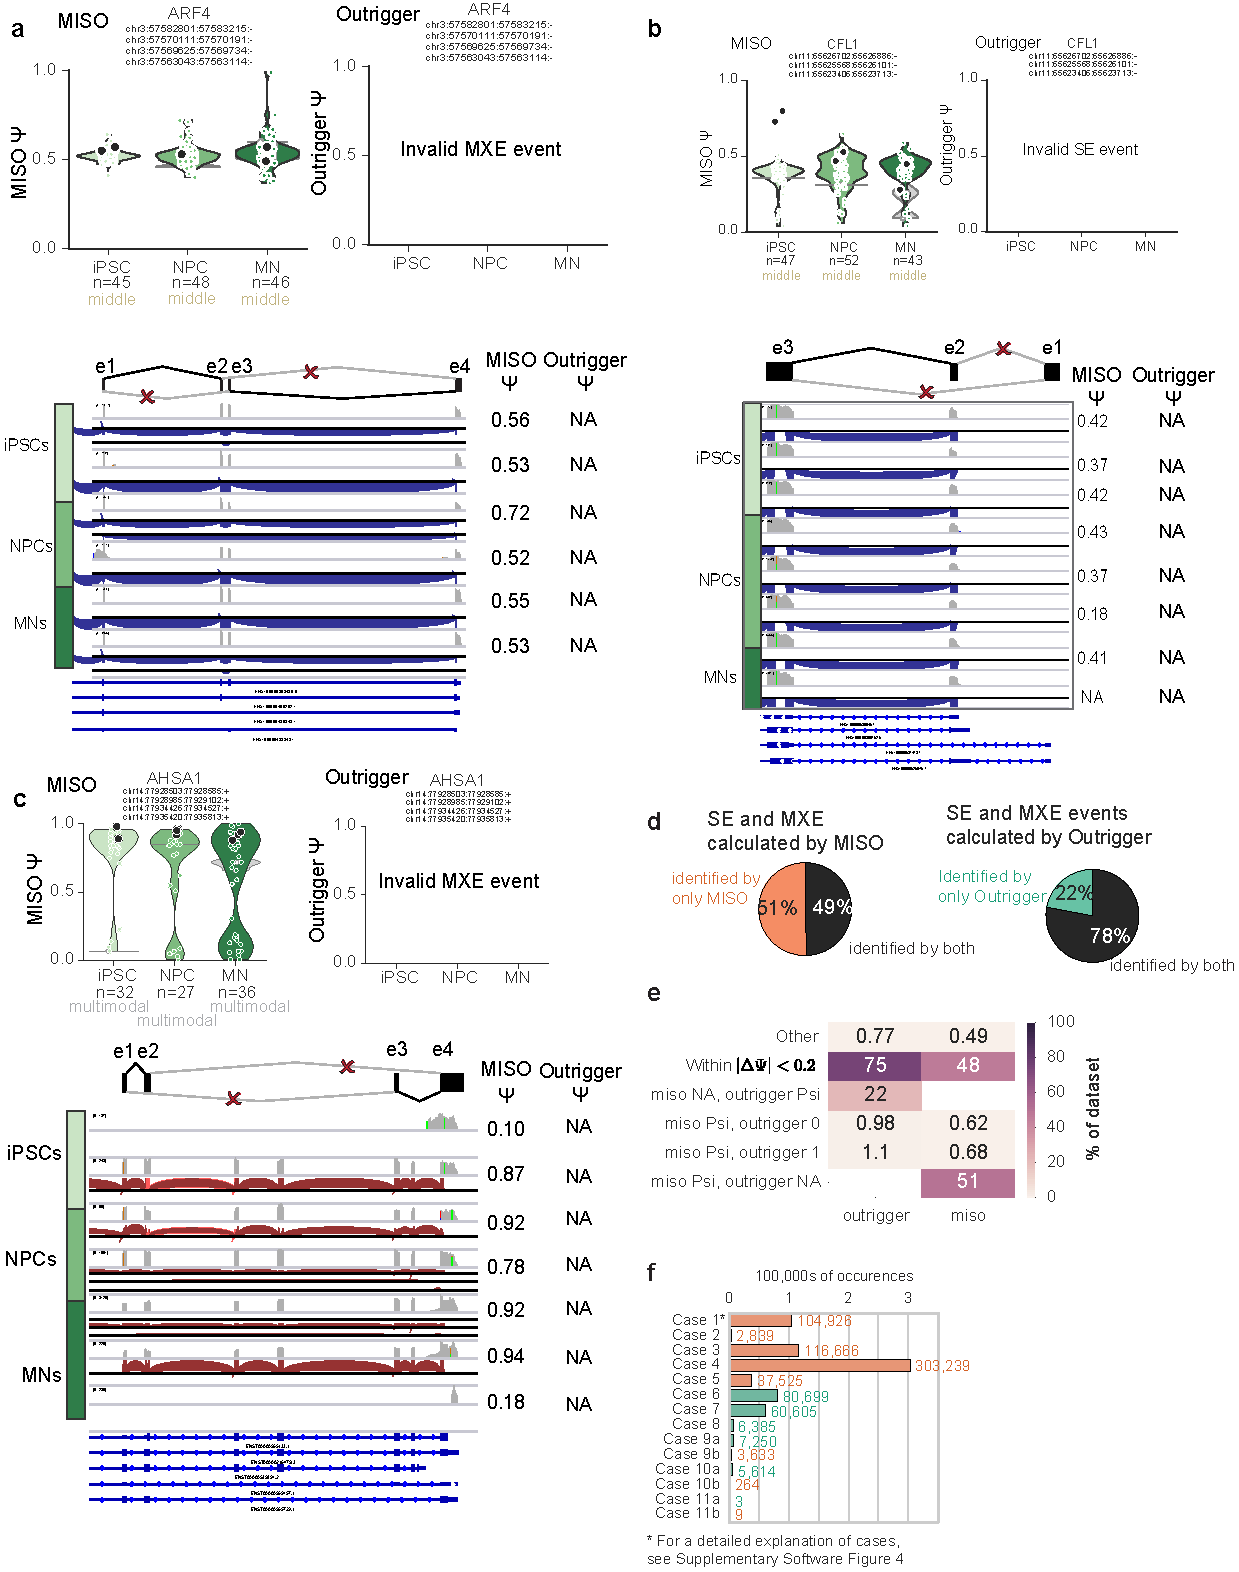
\includegraphics[width=5.8in]{figures/invalid_miso.pdf}
\end{figure}
%and, I'm not sure why, but one of the times I used this code the figure number wasn't augmented for the next figure, so check your figure numbers and if necessary uncomment the following line
%\addtocounter{figure}{1}
\clearpage
% --- END manual facingcaption for MISO fiugre --- %


The majority of the false positives are Case 4, where only one junction has sufficient reads. As MISO counts both junctions to calculate $\Psi$, shown in \textbf{\Cref{fig:miso}b-c}, many of the events are not covered on both sides of the alternative exons, which may suggest the events are not true SE events, but rather alternative first exon events, for instance.

We used MISO's event definitions and found that as many as 50\% of MISO events did not pass the stringent rules of \outrigger, primarily due to the incompatibility with the annotation of SE and MXE and insufficient coverage (\textbf{\Cref{fig:miso}j-l}).


\section{\texttt{anchor}: Modality estimation}
\label{sec:anchor}

\subsection{Algorithm overview}
\paragraph{Model modalities as beta distributions}

% \theoremstyle{definition}
We define \emph{modality} as a distinct type of distributions. Since $\Psi$s are continuous value between $(0, 1)$, distribution of $\Psi$ can be modeled as Beta distribution. The probability density function for the Beta distribution, $\mathrm{Pr}(\alpha, \beta)$ is defined between $(0, 1)$, with parameters $\alpha > 0$ and $\beta > 0$,

\begin{equation}
\mathrm{Pr}(\alpha, \beta) \sim \frac{1}{\mathrm{B}\left(\alpha, \beta\right)}  x^{(\alpha - 1)} \left(1-x\right)^{(\beta-1)},
\end{equation}

where $\mathrm{B}\left(\alpha, \beta\right)$ is the Beta function, defined by $\alpha > 0$ and $\beta > 0$. It may be easier to think about how the $\alpha$ and $\beta$ parameters affect distribution by observing the mean and variance \textbf{\Cref{fig:anchor_parameterization}a}. The beta distributions can be described by four parameterizations: $1 \leq \alpha < \beta$, $\alpha = \beta > 1$, $\alpha > \beta \geq 1$, $\alpha = \beta < 1$ (\textbf{\Cref{fig:anchor_parameterization}b}). Conveniently, these four configurations correspond to the four modalities we are interested in: $1 \leq \alpha < \beta$ corresponds to \emph{excluded}, $\alpha = \beta > 1$ to \emph{middle}, $\alpha > \beta \geq 1$ to \emph{included}, and $\alpha = \beta < 1$ to \emph{bimodal} (\textbf{\Cref{fig:anchor_parameterization}c}). The final \emph{multimodal} modality corresponds to $\alpha = \beta = 1$, which is equivalent to the uniform distribution used as null model.



\paragraph{Model parameterization}
To describe feature distribution as modalities, we parameterized the four parameterizable modalities and used Bayesian model selection to choose the best model to describe the distribution. Python package \texttt{scipy}\cite{Oliphant:2007dm,Millman:2011jv} was used to implement Beta distribution.
For \1 (\0) modality, we fixed $\beta$ ($\alpha$) at 1 and linearly increased $\alpha$ ($\beta$) from $2$ to $20$ (\Cref{fig:anchor_parameterization}d). We chose $2$ as a starting parameter since it is near the $\alpha=\beta=1$ uniform distribution, as we wanted to allow \0 and \1 distributions with noise. For bimodal (middle) modality, we changed $\alpha$ and $\beta$ simultaneously, monotonically decreasing (increasing) the parameters from $\alpha=\frac{1}{12}$, $\beta = \frac{1}{12}$ ($\alpha = 2, \beta = 2$) to $\alpha = \frac{1}{30}, \beta = \frac{1}{30}$ ($\alpha = 20, \beta=20$). The parameters for bimodal start at $\frac{1}{12}$ rather than $\frac{1}{2}$ because starting the parameters from $\frac{1}{2}$ resulted in more false positive ``bimodal'' events, whereas starting the parameters from $\frac{1}{2}$ ensures any density near $0.5$ is downweighted.


The fit of feature distribution is assessed to the four configurations using Bayes Factors, represented by $K$,

\begin{align}
K^{(m)}
&= \frac{P(D | M_1^{(m)})}{P(D | M_0)}\\
&=
\frac{\sum_{i} P(\alpha_i^{(m)}, \beta_i^{(m)} | M_i^{(m)}) P(D | \alpha_i^{(m)}, \beta_i^{(m)}, M_i^{(m)})}
{\sum P(\alpha_0, \beta_0 | M_0) P(D | \alpha_0, \beta_0, M_0)}\\
&=
\frac{\sum_{i} P(\alpha_i^{(m)}, \beta_i^{(m)} | M_i^{(m)}) P(D | \alpha_i^{(m)}, \beta_i^{(m)}, M_i^{(m)})}
{1}\\
&=
\sum_{i} P(\alpha_i^{(m)}, \beta_i^{(m)} | M_i^{(m)}) P(D | \alpha_i^{(m)}, \beta_i^{(m)}, M_i^{(m)})
\end{align}

Where $M_i^{(m)}$ is the model of interest (e.g. $M_i^{(\mathrm{bimodal})}$) and $\alpha_i^{(m)}, \beta_i^{(m)}$ are the corresponding parameters from the parameterization shown in \textbf{\Cref{fig:anchor_parameterization}d}. The null model, $M_0$ is the uniform distribution, where $\alpha_0 = \beta_0 = 1$, and thus $P(D|M_0) = 1$ for all datasets. We use a Bayes Factor cutoff of $K_{\mathrm{cutoff}}$ to indicate the threshold where the model begins to explain the data reasonably well. In practice we set $K_{\mathrm{cutoff}} = 2^{5}$ ($\log_2 K_\mathrm{cutoff} = 5$).

The \0 and \1 modalities vary only one parameter at a time, whereas middle and bimodal modalities vary both $\alpha$ and $\beta$ simoutanously. Models with more parameters are more likely to fit, thus we fit to the one-parameter models first, assessing whether $K > K_{\mathrm{cutoff}}$ for either \0 or \1. No distribution can fit both \0 and \1 modalities, thus it is assigned to the modality with highest $K$. Next, the distribution is fitted to the two-parameter bimodal and middle models, checking if $K > K_{\mathrm{cutoff}}$. If neither modality applies, we assign the modality to \emph{multimodal} (\textbf{2c}).

% --- BEGIN manual facingcaption for anchor_parameterization --- %
\clearpage
\thispagestyle{facingcaption}
\begin{figure}[h]
\captionsetup{labelformat=prev-page}
  \caption[Overview of \anchor\, parameterization of the Beta distribution.]{
  Overview of \anchor\, parameterization of the Beta distribution.\\
\textbf{a.}~Top, equation for the Beta distribution of the random variable $x$ with parameters $\alpha, \beta > 0$. Bottom left, equation for the mean ($\mu$) of the Beta distribution as a function of its parameters. Bottom right, equation for the variance ($\sigma^2$) of the Beta distribution as a function of parameters.\\
\textbf{b.}~Cartoon of valid values of $\alpha$ and $\beta$ parameters of Beta distribution, showing how the space is partitioned by the modalities.\\
\textbf{c.}~Violinplots representing the four ideal modalities, plus the null ``multimodal'' distribution. Each modality is annotated with examples of four cells representing within-cell distributions of included (dark grey) and excluded (light grey) transcripts, and the corresponding parameters of the Beta distribution.\\
\textbf{d.}~Violinplots of 1 million random samples of the family of Beta distributions specified by the $\alpha$ and $\beta$ ($x$ tick labels) parameterization of the four modalities: excluded, bimodal, included, and middle.}
\label{fig:anchor_parameterization}
\end{figure}
\clearpage
\begin{figure}[h]
\ContinuedFloat
\captionsetup{labelformat=empty}
\centering
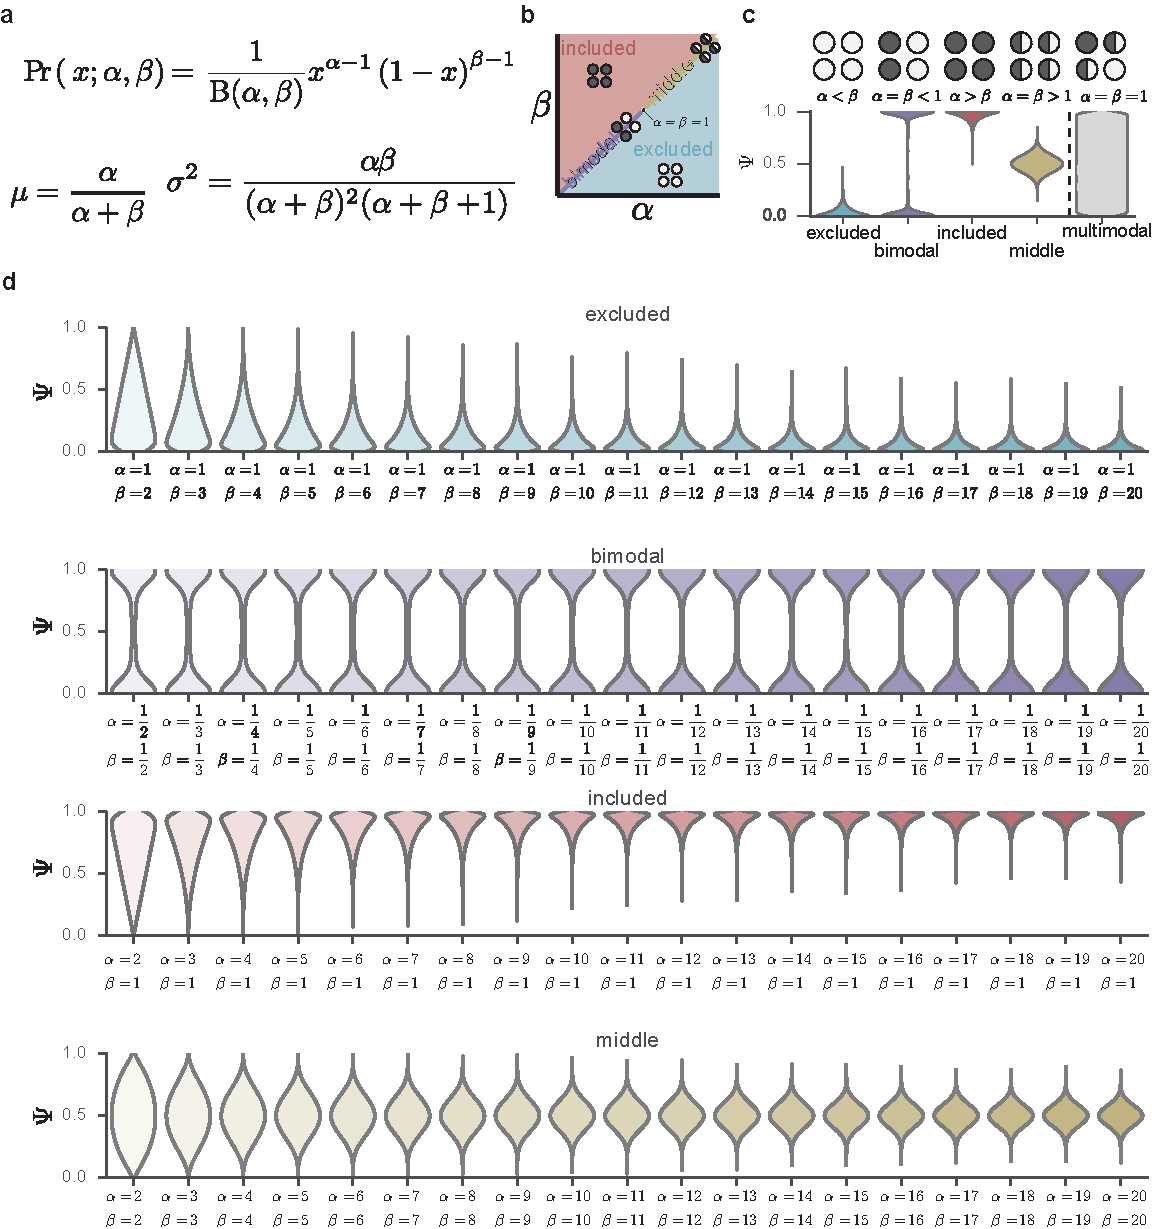
\includegraphics[width=5.8in]{figures/anchor_parameterization}
\end{figure}
%and, I'm not sure why, but one of the times I used this code the figure number wasn't augmented for the next figure, so check your figure numbers and if necessary uncomment the following line
\addtocounter{figure}{1}
\clearpage
% --- END manual facingcaption for anchor_parameterization --- %



As exact $0$ and $1$ are not in the range of the Beta distribution, we implement this model selection by adding a small number ($0.001$) to $0$ and subtracting this small number from $1$. Thus, we approximate the data-derived distribution from the invalid closed interval [0, 1] to the valid open interval of (0, 1).


\subsection{Simulations}

We optimized the algorithm parameters using test datasets and visually inspecting random samples from both the best- and worst-fitting data and ensuring that the even the worst fitting data was still believably categorized as the modality (\textbf{\Cref{fig:anchor_best_worst}}).

\paragraph{Dataset 1: ``Perfect Modalities'' with noise}
\label{sec:anchor_perfect_modalities}

To test the limits of \texttt{anchor}, we simulated perfectly \0, middle, \1, and bimodal distribution, added uniform random noise with 100 iterations, and estimated modality at each noise level with iteration (\textbf{\Cref{fig:anchor_simulations_perfect_modalities}a}). As expected, the most frequently predicted modality was ``multimodal,'' since the dataset was created from randomly added noise (\textbf{\Cref{fig:anchor_simulations_perfect_modalities}b}). The next frequent modality was bimodal, followed by a tie with excluded and included, and the least frequent one is middle modality. We found that these parameterizations can accurately predict modality with up to $35\%$ noise added to the middle modality, $50\%$ noise added to excluded and included modalities, and up to $70\%$ noise added to the bimodal modality(\textbf{\Cref{fig:anchor_simulations_perfect_modalities}d}). By visual inspection of distributions fit best or worst to each modality (\textbf{\Cref{fig:anchor_best_worst}a}), we observed that the bimodal distributions are sufficiently different from other parameterizations, demonstrating the robustness of the algorithm.



% --- BEGIN manual facingcaption for anchor best worst fits --- %
\clearpage
\thispagestyle{facingcaption}
\begin{figure}[h]
\captionsetup{labelformat=prev-page}
  \caption[Best and worst fitting modality data using \anchor.]{
  Best and worst fitting modality data using \anchor.\\
Left, 10 events with largest Bayes Factor, $K$ (best fit) from the assigned modality. Right, 10 events with smallest Bayes Factor, $K$ (worst fit) from their assigned modality. For multimodal, as there is no fit, this simply shows 20 random events.\\
\textbf{a.}~Bayesian \anchor\, method on ``Perfect modalities'' dataset.\\
\textbf{b.}~Bayesian \anchor\, method on ``Maybe bimodals'' dataset.
}
\label{fig:anchor_best_worst}
\end{figure}
\clearpage
\begin{figure}[h]
\ContinuedFloat
\captionsetup{labelformat=empty}
\centering
  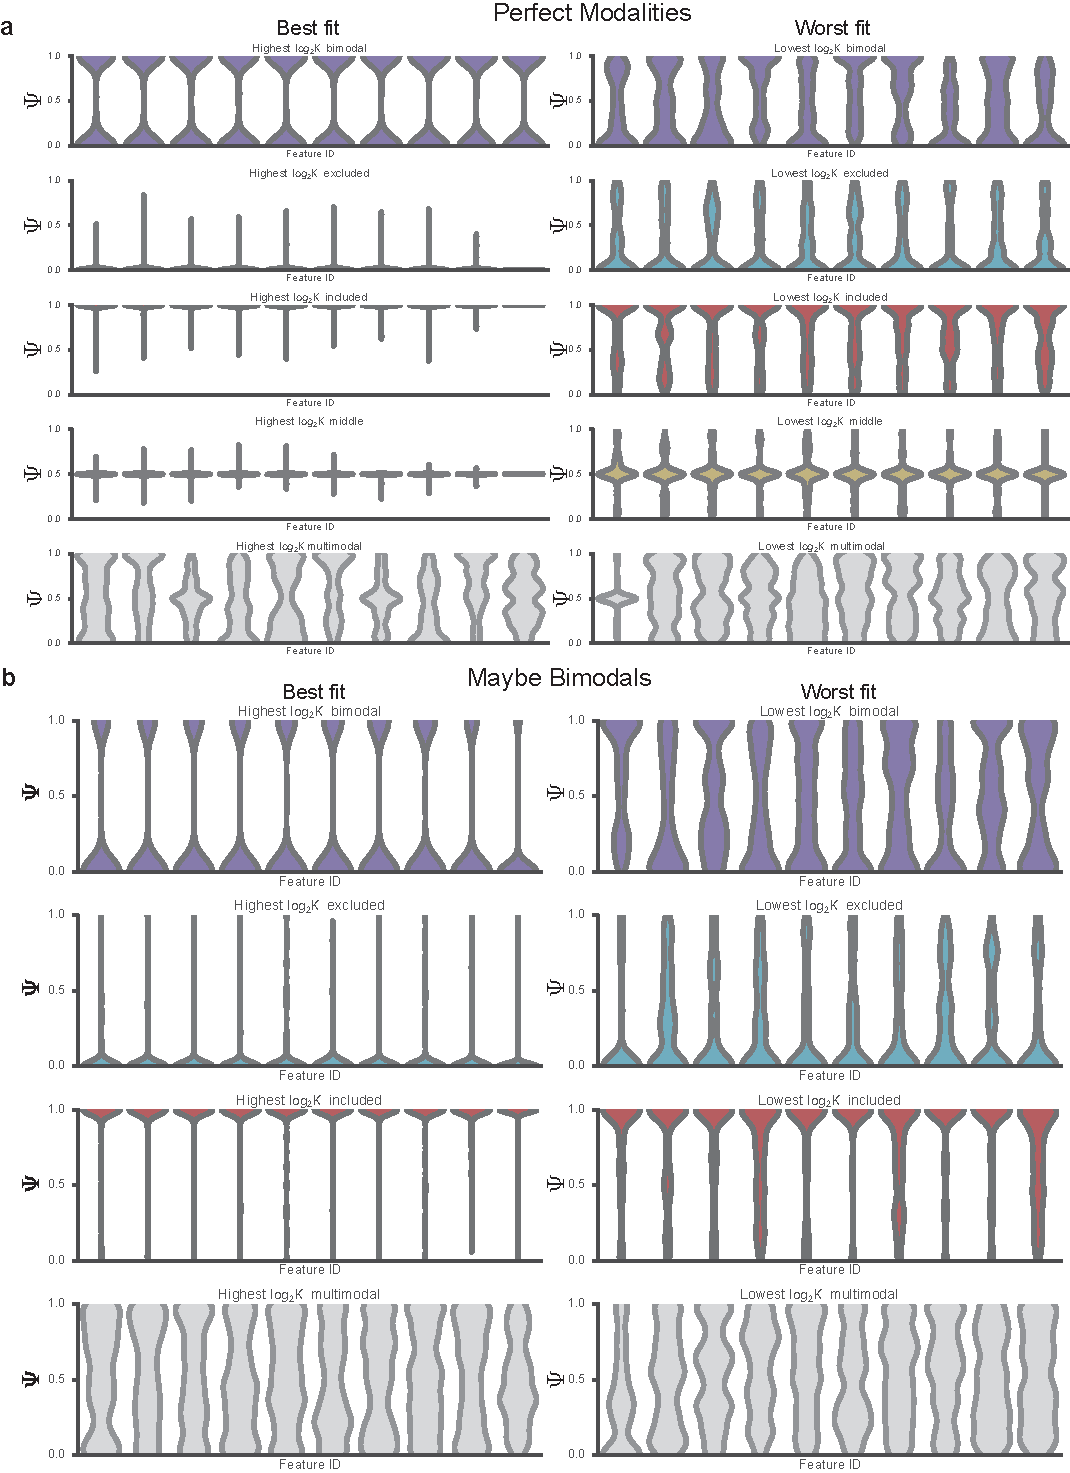
\includegraphics[width=5.8in]{figures/anchor_best_worst}
\end{figure}
%and, I'm not sure why, but one of the times I used this code the figure number wasn't augmented for the next figure, so check your figure numbers and if necessary uncomment the following line
\addtocounter{figure}{1}
\clearpage
% --- END manual facingcaption for anchor best worst fits --- %




% --- BEGIN manual facingcaption for perfect modalities anchor simulations --- %
\clearpage
\thispagestyle{facingcaption}
\begin{figure}[h]
\captionsetup{labelformat=prev-page}
\caption[Simulated ``Perfect Modality'' dataset to test performance of \texttt{anchor}.]{
Simulated dataset to test performance of \texttt{anchor}.\\
\textbf{a.}~Violinplots depicting the creation of simulated modality datasets with increasing noise. The base dataset (\% Noise = 0) consisted of 100 samples of either all zeros (excluded), half zeros and half ones (bimodal), all ones (included), or all $0.5$s (middle), exactly representing the four modalities. Uniform random noise was added in 5\% increments, with 100 iterations at each noise level.
\textbf{b.}~Percentage of events categorized as different modalities by \texttt{anchor} in the randomly generated test datasets, across all noise levels, as illustrated in (\textbf{a}). Number of events for each modality is annotated on top of the barplots. \\
\textbf{c.}~Percentage of events categorized as different modalities by binning in the randomly generated test datasets, across all noise levels, as illustrated in (\textbf{a}). Number of events for each modality is annotated on top of the barplots. \\
\textbf{d-g.}~Specificity of modality estimation. Recapitulation of the original modality as a function of additional noise, using \anchor\, (\textbf{d}), binning (\textbf{e}), Bimodality index (\textbf{f}), and diptest (\textbf{g}) methods. The $x$-axis depicts the percent of uniform random noise added (visualized as a triangle gradient), and the $y$-axis depicts the fraction of times a noisy feature was categorized into each modality. The hue of the line is the modality.
}
\label{fig:anchor_simulations_perfect_modalities}
\end{figure}
\clearpage
\begin{figure}[h]
\ContinuedFloat
\captionsetup{labelformat=empty}
\centering
% \includegraphics[width=5.8in]{sandiego.jpg}
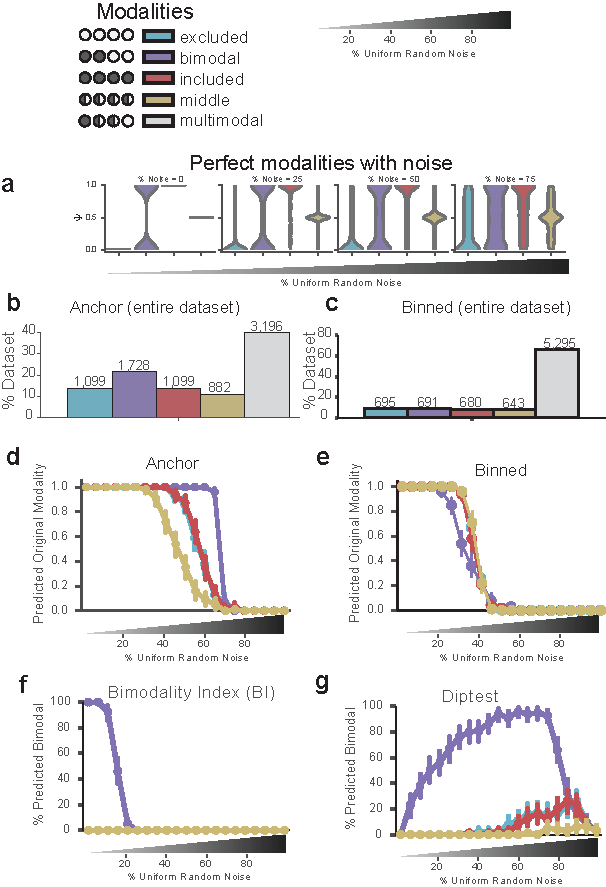
\includegraphics[width=5.8in]{figures/anchor_simulations_perfect_modalities.pdf}
\end{figure}
%and, I'm not sure why, but one of the times I used this code the figure number wasn't augmented for the next figure, so check your figure numbers and if necessary uncomment the following line
\addtocounter{figure}{1}
\clearpage
% --- END manual facingcaption for perfect modalities anchor simulations --- %


\paragraph{Dataset 2: ``Maybe Bimodals'' with noise}
\label{sec:anchor_maybe_bimodals}

To test the proportions of zeros and ones that able to constitute ``bimodal'' distribution, we created another dataset comprised 100 samples of varying amounts of 0s and 1s, and adding random uniform noise (\textbf{~\Cref{fig:anchor_simulations_maybe_bimodals}a}). The primary predicted modality was bimodal, then multimodal, and finally included and excluded (\textbf{Supplementary \Cref{fig:anchor_simulations_maybe_bimodals}b}). No distribution was predicted as the middle modality, indicating the bimodal and middle modalities are drastically different with little chance of mis-assignment. The falloff of correctly predicting bimodality is at adding $70\%$ noise (\textbf{Supplementary \Cref{fig:anchor_simulations_maybe_bimodals}b}), consistent with the previous simulation with ``Perfect Modalities'' dataset (\textbf{\Cref{fig:anchor_simulations_perfect_modalities}d}). We found that bimodality is determing with a 90:10 (10:90) proportion of samples of 0:1 (0:1) (\textbf{Supplementary \Cref{fig:anchor_simulations_maybe_bimodals}d}). Visual inspection of distributions fit best or worst to each modality confirmed the assignment of each modality(\textbf{\Cref{fig:anchor_best_worst}b}).

To summarize, simulation with two different datasets indicates that 1) bimodal modality can tolerate to up to $70\%$ of uniform random noise, and middle modality is least tolerable to noise at only $30\%$, 2) included and excluded modalities are drastically different, so as the middle and bimodal modalities, thus the two step modality assignment procedure (\textbf{Figure 2}) is well-grounded, 3) \anchor is able to determine a bimodal modality with up to 90:10 proportion of zeros and ones.



% --- BEGIN manual facingcaption for maybe bimodals anchor simulations --- %
\clearpage
\thispagestyle{facingcaption}
\begin{figure}[h]
\captionsetup{labelformat=prev-page}
\caption[Simulated ``Maybe Bimodals'' dataset to test performance of \texttt{anchor}.]{
Simulated bimodal dataset to test performance of \texttt{anchor}.\\
\textbf{a.}~Violinplots depicting the creation of the ``Maybe Bimodals'' test set consists of potential bimodal events, each containing 100 samples of only zeros ($\Psi = 0$) and ones ($\Psi = 1$) in every combination, shown here as relative to the number of ones. We added uniform random noise in increasing 5\% levels for 100 iterations at each level. While each combination of 1s and 0s was created, only a subset are shown for brevity -- 1:99, 25:75, 50:50, 75:25, and 99:1 ratios of 1:0 are shown, with added uniform random noise of 0\% (original), 25\%, 50\%, and 75\%.\\
\textbf{b.}~Percentage of events categorized in modalities by \texttt{anchor} in the randomly generated bimodal test datasets, across all noise levels, as illustrated in (\textbf{h}). Number of events for each modality is annotated on top of the barplots. \\
\textbf{c.}~Percentage of events categorized in modalities by binning in the randomly generated bimodal test datasets, across all noise levels, as illustrated in (\textbf{h}). Number of events for each modality is annotated on top of the barplots. \\
\textbf{d-k.}~Accuracy of bimodality prediction, as a function of the noise added to the dataset. \\
\textbf{d-g.}~Specificity of bimodality estimation upon addition of uniform random noise. The $x$-axis shows the percent added uniform random noise (visualized as a triangle gradient), and the $y$-axis indicates the fraction of time features in each noise percentage and proportion of $1:0$ was categorized as bimodal. Overall, all but the very extremes of the $1:0$ proportions were consistently categorized as bimodal until 70\% noise, after which point nearly all events became multimodal. Modality estimations are shown using \anchor\, (\textbf{k}), binning (\textbf{l}), Bimodality Index (\textbf{m}), and Diptest (\textbf{n}).\\
\textbf{h-k.}~Sensitivity of bimodality detection. Percentage of events predicted as bimodal given different proportions of 0s and 1s, and increasing uniform random noise. Events are called as bimodal with approximately 9:1 ratio of 0s and 1s (and vice versa), shown with a dotted line at 10\% ones and 90\% ones. Bottom triangle gradient shows increasing ratio of ones to zeros, i.e. from exclusion to bimodal, to inclusion. Bimodality estimations are shown using \anchor\, (\textbf{o}), binning (\textbf{p}), Bimodality Index (\textbf{q}), and Diptest (\textbf{r}).
}
\label{fig:anchor_simulations_maybe_bimodals}
\end{figure}
\clearpage
\begin{figure}[h]
\ContinuedFloat
\captionsetup{labelformat=empty}
\centering
% \includegraphics[width=5.8in]{sandiego.jpg}
\includegraphics[height=8in]{figures/anchor_simulations_maybe_bimodals.pdf}
\end{figure}
%and, I'm not sure why, but one of the times I used this code the figure number wasn't augmented for the next figure, so check your figure numbers and if necessary uncomment the following line
\addtocounter{figure}{1}
\clearpage
% --- END manual facingcaption for maybe bimodals anchor simulations --- %


\subsection{Comparison to other methods}

\paragraph{Simple binning}
We can compare this to other methods we attempted, such as fixing bins of $[0, 0.3, 0.7, 1]$ and using cutoffs for the densities, which does not account for the continuous nature of the underlying distributions. We found the modality whose binned distribution was the smallest distance (measured by Jensen-Shannon Divergence \cite{Cover:2011vn}) away from each binned event. In both the simulated modalities and simulated bimodal datasets, we found a sharp increase in multimodal distributions and by eye, poorer categorization of the bimodal modality, especially at the decision boundary of low JSD (\textbf{Figures~\cref{fig:anchor_simulations_maybe_bimodals}c, e, j, l, p}).

% \paragraph{Fitting a Beta distribution to individual features}

% or fitting a Beta distribution to each individual feature (which takes a long time) and using cutoffs on the estimated parameters, which is also problematic and error-prone.

\paragraph{Bimodality index}
Another test for bimodality is the Bimodality Index \cite{Wang:2009wm} (BI), which requires estimating each feature as a mixture of Gaussian models. We used the implementation of Generalized Mixture Models in \texttt{scikit-learn} \cite{Pedregosa:2011tv} to estimate two Gaussian distributions for each model, and calculated the BI. For perfect bimodal featues, the value is large, for example, we found that for the zero-noise bimodal event, the $\mathrm{BI}=402$) and was the single bimodality index that was larger than $100$ for any feature (\Cref{fig:anchor_simulations_maybe_bimodals}f, j). This shows that our method is more sensitive to finding bimodal features with the addition of noise, which BI cannot handle.

\paragraph{Hartigan's Dip test}
A commonly used test for unimodality is Hartigan's dip test\cite{Hartigan:1985ca}. If the distribution fails the unimodality test, then it is considered bimodal. To define a cutoff for when the dip statistic becomes reliable, we calculated the dip statistic using a Python implementation of the test, called \texttt{diptest}\cite{Anonymous:zTNIPlgQ}. We used a $p$-value cutoff of $p <0.05$ as our threshold for assigning an event as bimodal. We used the diptest statistic on the two datasets, and found that while the zero-noise bimodal event was not detected as bimodal, adding as small amount of noise \emph{improved} the diptest's detection of bimodal events (\textbf{\Cref{fig:anchor_simulations_maybe_bimodals}g,k}), and the accuracy dropped off at a very high noise level - 90\%. As expected, the excluded, included, and middle modalities weren't detected as bimodal, except at higher noise levels, which we also saw with \anchor.


\section{\texttt{bonvoyage}: Transformation of distributions to \emph{waypoints} and \emph{voyages}}
\label{sec:bonvoyage}

\subsection{Algorithm overview}

The goal of \bonvoyage\, is to be able to summarize the entire distribution of a feature into a single point in space, enabling visualization multiple distributions at a time with intuitive interpretation. To accomplish this, we will transform one-dimensional vectors into two-dimensional space. Specifically, the $x$-axis will represent the \emph{excluded} dimension and the $y$-axis will represent the \emph{included} dimension, and all points will be described as a sum of \0 and \1 components (\textbf{6a}, left). For example, for two distinct cell-types, we can imagine a feature that starts at a \1 modality in the first and changes to a \0 event in the second, or changes from middle to bimodal (\textbf{6a}, right).



\paragraph{Data discretization}
We will use a reduced representation of our splicing data by binning each feature on bins $b$ of size $0.1$, where $b_n$ represents the $n$th bin. We represent the binned splicing matrix with $B_\Psi$, where $B_\Psi[k,j]$ represents the fraction of non-null samples in feature $j$ with $\Psi$ value contained in $b_k$. In practice, we pre-filter the data by using only features for which there are enough samples. In the main text for this paper, we used a minimum of 10 cells.

\paragraph{Dimensionality reduction via non-negative matrix factorization}
Non\hyp{}negative matrix factorization (NMF) is a parts\hyp{}based dimensionality reduction algorithm which results in meaningful, interpretable results \cite{Lee:1999gw}. It is an alternative to other dimensionality reduction methods such as principal- and independent- component analyses (PCA and ICA) because its features are both independent, and non-negative, and thus each feature is composed of a sum of the underlying structure of the data, without pesky negative terms.

Thus, for NMF, we will be reducing $B_\Psi$ as such,

\begin{equation}
B_\Psi \approx W \times H,
\end{equation}

Where $W$ is a (features, $2$)-size matrix of the composition of each feature as a sum of how many samples are excluded and included. We found that in the alternative splicing data, the primary components were the included and excluded values, but in other datasets, this may not be the case. Thus, as the components of NMF are the most prominent features, to ensure reproducibility of the axes across datasets, we seeded the NMF transformation with a matrix that is composed of features that are primarily \0 plus a single \1 feature. We used the Python package \texttt{scikit-learn} \cite{Pedregosa:2011tv} for the Projected Gradient NMF implementation.

We call the projected distributions ``waypoint space,'' and the distance between two points a ``voyage,'' such as the voyage of the MXE event in PKM (\Cref{fig:bonvoyage_overview}c).

% For multiple cell-types, we as we will show in the simulations (the next section, \Cref{subsubsec:bonvoyage_simulations}), we \emph{could} plot all voyages as arrows, but for many at a time, it can be easier to visualize through a hexagonally binned scatterplot, where the $x$-axis is the $\Delta$excluded axis, and the $y$-axis represents the $\Delta$included axis.

\subsection{Simulations}
\label{subsubsec:bonvoyage_simulations}



% The goal of \texttt{bonvoyage} is to identify features which change across groups. As diagrammed in \Cref{fig:example_feature}, the idea is to transform distributions of values into a single point onto \emph{waypoint space}, find the distances between transformed distributions and plot the vectors onto \emph{voyage space}.

\paragraph{Transformation of static distributions}

To demonstrate the ability of\linebreak \texttt{bonvoyage}, we created a simulated dataset which we call ``Maybe Everything'' consisting of every combination of 0s, 1s, and 0.5s (\Cref{fig:bonvoyage_simulations}a-d), essentially incorporating both the ``Perfect Modalities'' (from \Cref{sec:anchor_perfect_modalities}) and ``Maybe Bimodals'' (from \Cref{sec:anchor_maybe_bimodals}) into a single dataset. Again, we added uniform random noise at $5\%$ intervals. We transformed the entire simulated dataset into the \emph{``waypoint''} space.


To identifying features which change in distribution, we calculate the \emph{``voyage''} between them in waypoint space. As a demonstration, we shuffle the simulated data to create two different \emph{in silico} phenotypes. We will use each feature as a \emph{``waypoint''} along the voyage, and calculate total travel distance of each feature between the phenotypes.


A key aspect of the waypoint space is that while changes from exclusion to inclusion are easy to spot by a change in means, the change from a middle to a bimodal is not, and requires a battery of other tests to find. Here, voyage space has a significant advantage as it gives both the magnitude of change and a directly interpretable direction.

% --- BEGIN manual facingcaption for bonvoyage simulations --- %
\clearpage
\thispagestyle{facingcaption}
\begin{figure}[h]
\captionsetup{labelformat=prev-page}
\caption[Visualization capabilities of \bonvoyage\, shown with simulated data.]{Visualization capabilities of \bonvoyage\, shown with simulated data\\
\textbf{a-d.}~Datasets used for testing \bonvoyage. Uniform random noise was added in 5\% intervals to all datasets, up to 95\% noise, for 100 iterations at each noise level.\\
\textbf{a.}~Perfect middle, included, and excluded modalities, with added noise. Only 0\%, 25\%, 50\% and 75\% noise levels are shown for brevity. Top, averaged violinplots for all features at a given level of noise. Bottom, waypoint space of all features at the specified noise level.\\
\textbf{b.}~Maybe middle-included modalities, created with every combination of $0.5$ and $1.0$ values. Only the 0\% noise dataset is shown for brevity. Top, violinplots, bottom, waypoint plots.\\
\textbf{c.}~Maybe excluded-middle modalities, created with every combination of $0.0$ and $0.5$ values. Only the 0\% noise dataset is shown for brevity. Top, violinplots, bottom, waypoint plots.\\
\textbf{d.}~Maybe bimodal modalities, created with every combination of $0$ and $1$ values. Only the 0\% noise dataset is shown for brevity. Top, violinplots, bottom, waypoint plots.\\
\textbf{e.}~Comparison of voyage magnitude and JSD between ``Maybe everything'' data and a shuffled copy to show the entire distribution.
}
\label{fig:bonvoyage_simulations}
\end{figure}
\clearpage
\begin{figure}[h]
\ContinuedFloat
\captionsetup{labelformat=empty}
\centering
% \includegraphics[width=5.8in]{sandiego.jpg}
  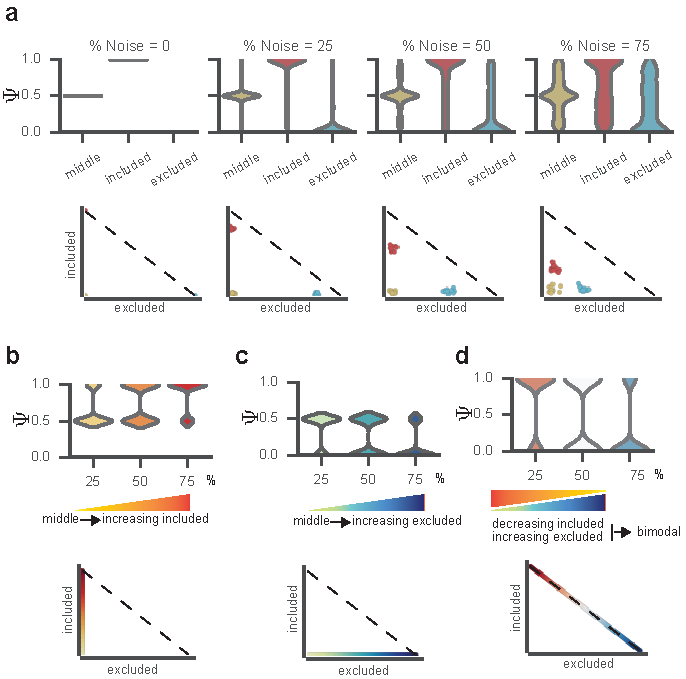
\includegraphics[width=5.8in]{figures/bonvoyage_simulations}
\end{figure}
%and, I'm not sure why, but one of the times I used this code the figure number wasn't augmented for the next figure, so check your figure numbers and if necessary uncomment the following line
\addtocounter{figure}{1}
\clearpage
% --- END manual facingcaption for bonvoyage simulations --- %

\subsection{Comparison to other methods}

As there exist many methods for comparing distributions, we will show that the magnitude of change obtained from \texttt{bonvoyage} is comparable to other metrics for assessing changes in distribution. In particular, we will show the metrics within each modality, and across modalities, compared to Jensen-Shannon Divergence \cite{Cover:2011vn} (JSD) in (\Cref{fig:bonvoyage_simulations}). While JSD is more sensitive to slight changes in distribution (their scatterplots are skewed towards the right), it does not also encode directionality of change. Thus, \texttt{bonvoyage} offers a unique perspective on how to interpret changes in distribution.

\section{Acknowledgements}

Chapter 2, in part, has been accepted for publication as the supplementary material as it may appear in Molecular Cell, 2017, Yan Song$^*$, Olga B Botvinnik$^*$, Michael T Lovci, Boyko Kakaradov, Patrick Liu, Jia L. Xu and Gene W Yeo ($^*$ These authors contributed equally to this work).  The dissertation author was one of the primary investigators and authors of this paper. 
%
% Of course, if you prefer, you can just start with
%   \chapter{My First Chapter Name}
% and start typing away.  
\chapter{Just a Test}
This is only a test.
\section{A section}
\index{latin}Lorem ipsum dolor sit amet, consectetuer adipiscing elit. Nulla odio
sem, bibendum ut, aliquam ac, facilisis id, tellus. Nam posuere pede
sit amet ipsum. Etiam dolor. In sodales eros quis pede.  Quisque sed
nulla et ligula vulputate lacinia. In venenatis, ligula id semper
feugiat, ligula odio adipiscing libero, eget mollis nunc erat id orci.
Nullam ante dolor, rutrum eget, vestibulum euismod, pulvinar at, nibh.
In sapien. Quisque ut arcu. Suspendisse potenti. Cras consequat cursus
nulla.
\subsection{More Stuff}
Blah

\chapter{How to Recognise Different Types of Trees From Quite a Long Way Away}

\section{No. 1, the Larch}
\begin{figure}[ht] 
  \centering
  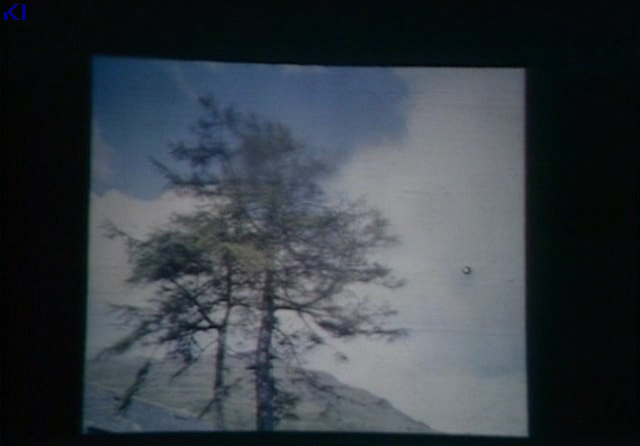
\includegraphics[width=0.8\textwidth]{larch}
  \caption{Shown is a picture of the larch as might be seen from quite a long way away.\index{Larch}}
\end{figure}

\section{And Now . . . No. 1, the Larch}
\newpage
\thispagestyle{facingcaption}
\begin{center}
\vspace*{3in}
\textbf{Figure \ref{Sideways Larch}:} Here is a caption for the Larch after you have had a wee too much to drink.

\end{center}
\newpage

\begin{figure}[hb] 
  \centering
  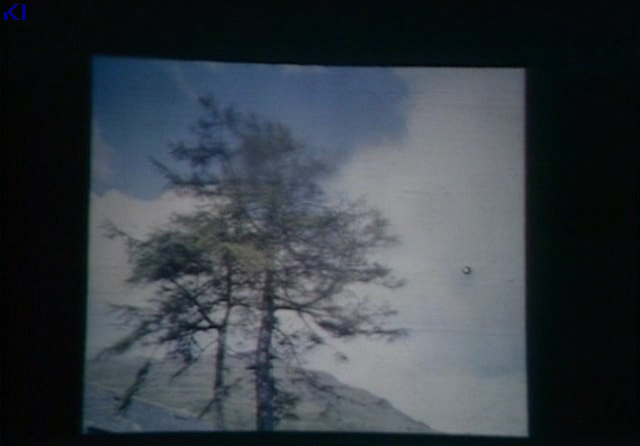
\includegraphics[width=0.8\textwidth]{larch}
  \caption[No. 1 The Larch]{Shown is a picture of the larch as might be seen from quite a long way away.\index{Larch}}\label{Sideways Larch}
\end{figure}

% Here I am testing that page breaking on the TOC works correctly.
% We never want the page break directly after a chapter entry.
\chapter{Another chapter}
\section{Some Stuff You Probably Don't Want to Read}
\section{Some Stuff You Really Don't Want to Read, it is Utterly and Completely Dull}
%\section{Now I am Just Writing Filler}
%\section{More Filler}
%\subsection{How Many Lines Am I at?}
%\subsection{Stuff}
%\section{Stuff}
%\section{Ooo-De-Laly}
%\subsection{Ooo-De-Laly, Ooo-De-Laly}
%\section{Slithy Toves}


\chapter{On the Inner Workings of a Grad Student Mind}
\section{Before Thesis Writing Has Begun}
\section{During Thesis Writing}
\section{During Thesis Formatting}
\section{After Thesis Writing}
\section{Before Defense}
\section{After Defense}

The Mock Turtle sighed deeply, and drew the back of one flapper across his eyes. He looked at Alice, and tried to speak, but for a minute or two sobs choked his voice. `Same as if he had a bone in his throat,' said the Gryphon: and it set to work shaking him and punching him in the back. At last the Mock Turtle recovered his voice, and, with tears running down his cheeks, he went on again:


\begin{verbatim}
``There's a porpoise close behind us, and he's treading on my tail.
See how eagerly the lobsters and the turtles all advance!
They are waiting on the shingle--will you come and join the dance?

Will you, won't you, 
                will you, won't you, 
                                will you join the dance?
Will you, won't you, 
                will you, won't you, 
                                won't you join the dance?''
\end{verbatim}



So Alice began telling them her adventures from the time when she first saw the White Rabbit. She was a little nervous about it just at first, the two creatures got so close to her, one on each side, and opened their eyes and mouths so very wide, but she gained courage as she went on. Her listeners were perfectly quiet till she got to the part about her repeating `You are Old, Father William,' to the Caterpillar\footnote{Which we introduced in a different thesis}, and the words all coming different, and then the Mock Turtle drew a long breath, and said `That's very curious'.

\appendix
\chapter{Final notes}
  Remove me in case of abdominal pain.





%% END MATTER
\printindex %% Uncomment to display the index
% \nocite{}  %% Put any references that you want to include in the bib 
%               but haven't cited in the braces.
% \bibliographystyle{alpha}  %% This is just my personal favorite style. 
%                              There are many others.
% \bibliography{myrefs}  %% This looks for the bibliography in myrefs.bib 
%                          which should be formatted as a bibtex file.
\end{document}

